\documentclass[notitlepage, prx, preprint, amsmath,superscriptaddress,amssymb]{revtex4-1}

\usepackage{subfigure,dcolumn}
\usepackage[T2A,T1]{fontenc}
\usepackage[english]{babel}
\usepackage{braket}
\usepackage{graphicx}
\usepackage[colorinlistoftodos]{todonotes}
\usepackage[utf8]{inputenc}
\usepackage{amsthm}

%%%%% to show the label in the Eqs.
\usepackage[notref,notcite]{showkeys}

%%%%%% theorems
\newtheorem{theorem}{Theorem}[section]
\newtheorem{lemma}{Lemma}[section]
\newtheorem{corollary}{Corollary}[section]




%%%%%%%%%%%%%%%%%%%%%
%%%%%%%%%%%%%%%%%%%%%
%%%%%%%%%%%%%%%%%%%%%
\begin{document}


\title{Causality and the N-photon Scattering matrix in waveguide QED}

\author{E. S\'anchez-Burillo}
\affiliation{Instituto de Ciencia de Materiales de Aragon and Departamento de Fisica de la Materia Condensada, CSIC-Universidad de Zaragoza, E-50012 Zaragoza, Spain}

\author{A. Cadarso}
\affiliation{Instituto de Fisica Fundamental, IFF-CSIC, Calle Serrano
  113b, Madrid E-28006, Spain}

\author{L. Mart\'in-Moreno}
\affiliation{Instituto de Ciencia de Materiales de Aragon and
  Departamento de Fisica de la Materia Condensada, CSIC-Universidad de
  Zaragoza, E-50012 Zaragoza, Spain}

\author{J. J. Garc\'ia-Ripoll}
\affiliation{Instituto de Fisica Fundamental, IFF-CSIC, Calle Serrano
  113b, Madrid E-28006, Spain}

\author{D. Zueco}
\affiliation{Instituto de Ciencia de Materiales de Aragon and Departamento de Fisica de la Materia Condensada, CSIC-Universidad de Zaragoza, E-50012 Zaragoza, Spain}
\affiliation{Fundacion ARAID, Paseo Maria Agustin 36, E-50004 Zaragoza, Spain}



\begin{abstract}
$S^0$ under general conditions.
\end{abstract}



\maketitle

\section{Introduction}


{\color{red}
To say:

decimos explictamente algo sobre que con RWA el g.s. es trivial y todo sale igual que aqui?


creo que alguna cita a Baranguer habria que poner (tiene seminal de two photon S-matrix? La de quantum computing en technological applications).

}

Causality is  expected to hold in every circumstance.    In words of Weinberg, two uncorrelated experiments must provide uncorrelated results \cite{Weinberg1996}.     In Quantum Field Theory, causality imposes that  spacelike-separated operators conmute.   In non-relativistic quantum mechanics, however, we should abandon such an stringent condition which  does not imply causality violation.  In local Hamiltonians~\footnote{interactions decay sufficiently fast with the distance}, there is a finite maximum  group velocity at which the information can travel.   Although operators do not conmute,  their conmutator  (its norm) is arbitrarily small at distances large enough compared to this maximum velocity  bounded by Lieb and Robinson \cite{Lieb1972}.  

Lieb-Robinson bounds  brought about that several rigorous results in QFT  were verified in many body quantum mechanics such as the exponential decay of correlations (at equilibrium)  in gapped models or  the area law \cite{Nachtergaele2006, Hastings2007}.   Another key object  to look at is the scattering matrix.  Scattering experiments  are the way we probe systems.  Experiments dictate the acceptable form for the $S$-matrix.  At the most fundamental level, causality imposes that the output for  uncorrelated inputs must be the sum of each of them in a convenient way.   Under some conditions (discussed below) the sum it is reduced to a  cluster decomposition \cite{Wichmann1963}.   
In fact,  acceptable QFT interactions  can be argued by imposing such a decomposition   \cite[Chap. 4]{weinberg1995}.   
It may be desirable to proof such a decomposition in non-relativistic many body systems.  On the other hand, it should not be  surprising that such a thing occurs, as we have just reviewed, a maximum velocity for transfer quantum information guarantees causality.  Checking this expected result is the purpose of this paper.

In particular, we consider the situation  occurring in  waveguide QED,  where travelling photons interact with local quantum systems.   In general, the photonic medium will be dispersive
{\color{red} dispersive = absorving?} and the coupling with the quantum systems may be non-perturbative.  In this sense, the problem we tackle is a many body one.  Besides,  typical (QFT) assumptions as Lorentz or translational invariance cannot be done here.  Although  motivated from a fundamental perspective, it is worth recallying that our work is experimentally  and technologically relevant nowadays \cite{lodahl15review}.
Physical implementations based on dielectric \cite{Mitsch2014, Yu2014}, cavity arrays \cite{Vuckovic2003}, metals  \cite{Lukin2007} or superconductors \cite{astafiev10, hoi11, Liu2016, Forn-Diaz2016} interacting with atoms, molecules,  q-dots or superconducting qubits constitute already an extense zoo to investigate the few photon scattering in the quantum domain. 
Thus,  waveguide QED experiments can test such causality restrictions for the $S$-matrix. 
Maybe driven by  the experimental interest, it exists already a large  theoretical literature for  waveguide QED systems \cite{Roy2016}  and in  computing the $N$-photon $S$-matrix in particular {\color{red} relevant citations}.  Our work is also of interest there, since derives from the most fundamental level the actual form of the $S$-matrix in all these platforms.



Our main result is the form for  the $N$-photon $S$-matrix  fixed by causality.   The result needs for intermediate  theorems stating what causality means  in the photonic medium  and the conditions for the existence for the $S$-matrix.  Our results do not rely on  approximations as Markovian and/or weak scatterer-photonic medium coupling. Thet are also independent of the scatterer.   Thus, our results are rather general.    
Finally, our theory is applied to  two examples where, either analytically (the case of  a non-dispersive medium interacting with a lambda atom \cite{Xu2016}) or numerically (scattering in the ultrastrong limit \cite{Sanchez-Burillo2014, Sanchez-Burillo2015}) has been recently discussed in the literature.   Both models share the property of  presenting Raman scattering which introduces several subtleties that we will discuss. 


The rest of the paper...


FRASES SUELTAS

*******

In any case, it would be desirable to extract whose properties must satisfy the matrix irrespective of the details of the model.   In top of that it is appealing to fix the outcomes just by minimal assumptions and/or understand how a basic paradigm as causality appears in waveguide QED experiments.  

Even it those cases where analytical tools are available the actual computation is quite cumbersome [citas]. 

*******

\section{Model, $S$-matrix and main results} 

{\color{red}TENEMOS QUE CAMBIAR LA NOTACIÓN DE LOS OPERADORES DE INTEARCCIÓN $S$. ESA LETRA ES PARA LA MATRIZ DE SCATTERING}

In waveguide QED the relevant model is  $(\hbar=1)$, 
\begin{equation}
H = \int \; d k  \, \omega_k \, a_k^\dagger a_k + H_{sys} + \int \; dk  \,  g_k  \, (S^\dagger a_k + S a_k^\dagger).
%H = \sum_k \omega_k a_k^\dagger a_k + H_{sys} + \sum_k g_k (S^\dagger a_k + %S a_k^\dagger).
\label{H-full}
\end{equation}
where $\omega_k$ are the photon frequencies and $a_k$ ($a_k^\dagger$) are bosonic operators, $[a_k, a_{k^\prime}^\dagger]= \delta (k - k^\prime)$.
We assume a single photon band:  $\omega_k \in [\omega_-, \omega_+]$  (multiband systems do not modify our conclusions). 
%Besides,  $k = n \pi /L$ with $n=-L/2, ..., 0, ... L/2$, \emph{i.e.} with momentum spacing $\delta_k = \pi / L$.  
The system and bosons couple via the operator $S$. The strength of the interaction is given by  $g_k$.   $H_{sys}$ is the system Hamiltonian that can be any.  
Actual calculations are fixed to one quantum system.  The extension to several scatterers  is trivial and do not change our findings.   When transforming to real space,
\begin{equation}
\label{axak}
a_x = \frac{1}{\sqrt{2 \pi } } \int \; d k   \, e^{i k x} a_k  
\end{equation}
the punctual scatterer is assumed to occupy a finite number of sites, \emph{i.e.} $g_x = 1/\sqrt{2 \pi } \int \; dk  e^{i k x} g_k$ has a finite support of size $m$. 
%is different from zero only sites $x=0, 1, ..., m$ with $m$ the ``size'' of the scatterer. 
 %If necessary,  the continuum limit of the model can be done with the replacements $\sum_k \to \int  dk$ via $a_k \to \sqrt{\delta_k} a(k)$ ($[a (k), a^\dagger (k^\prime)]= \delta(k-k^\prime)$) and $g_k \to \sqrt{\delta_k} g(k)$. 
No more assumptions on the model  will  invoked to prove our results, making our statements rather general. It is worth to insist that \eqref{H-full} models all the experimental implementation enumerated in the introduction.


We are interested in discussing the scattering wich is characterised by the $S$-matrix, relating the input and the output, defined as,
\begin{equation}
\label{Sdef}
( S_{y_1 ...y_n x_1...x_N} )_{\mu \nu} = \langle \mu | \langle y_1, ..., y_N | \lim_{t_\mp  \to \mp \infty} U_I(t_-, t_+) | x_1, ..., x_N \rangle | \nu \rangle
\end{equation}
Here,  $U_I(t_-, t_+)= e^{i H_0 t_-} \,  e^{-i H (t_+- t_-)}  \,  e^{-i H_0 t_+}$ is the evolution operator  in the interaction picture ($H_0=  \int \; d k  \, \omega_k \, a_k^\dagger a_k $).
Besides, $|x_1, ...,x_N\rangle$ ( $|y_1, ...,y_N\rangle$)  are  position eigenstates in the $N$-photon subspace,  $|\nu \rangle$  ($|\mu\rangle$) {\color{blue} estable?} eigenstates of the scatterer and $U (t_-, t_+) = e^{-i H (t_+-t_-)}$ is the evolution operator.  
It is clear that being \eqref{H-full} an inherent quantum many body problem, its evolution and thus the $S$-matrix is only solvable in some particular instances [ ], or with  approximations [] or numerically [].    

  
%%%%%%%%%%%%%%%
\begin{figure}
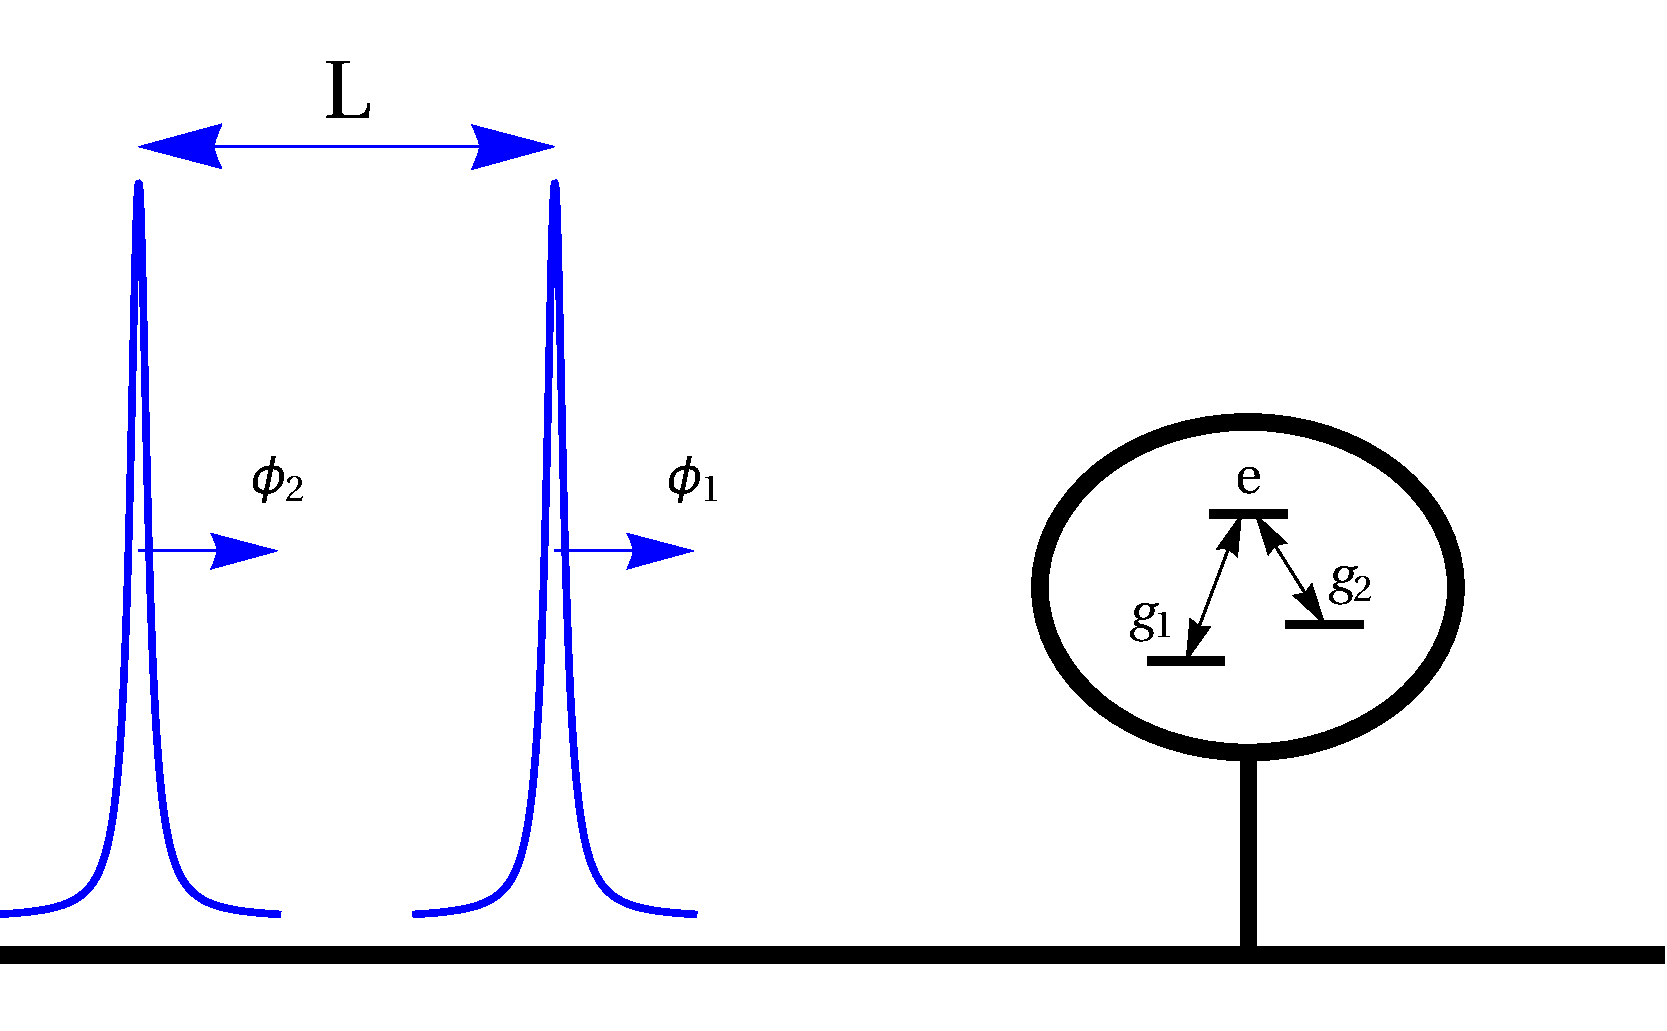
\includegraphics[scale=0.25]{input.pdf}
\caption{Two-photon input state impinging on a $\lambda$ atom. The state $\ket{e}$ is an unstable state which decays to the stable ones, $|g_1\rangle$ and $|g_2\rangle$. The distance $L$ between both wave packets, $\phi_1$ and $\phi_2$, will eventually tend to $\infty$.}
\label{fig:input}
\end{figure}

%%%%%%%%%%%%%%%




\subsection{Main results}

 Irrespective of the  model details  we show here that  it is possible to \emph{show} that within the light-matter Hamiltonian \eqref{H-full} whenever $|x_i -x_j| \to \infty$ and $|y_i -y_j| \to \infty$, then
\begin{equation}
\label{S0-main}
( S_{y_1 ...y_n x_1...x_N} )_{\mu \nu} \to
\sum_{\lambda_1\dots \lambda_{N-1}=1}^M\prod_{n=1}^N (S_{y_nx_n})_{\lambda_{n-1}\lambda_n}
\prod_{m=1}^{N-1}\theta(y_{m+1}-y_m) + \text{permutations},
\end{equation}
with $\lambda_0\equiv \mu$ and $\lambda_N\equiv\nu$.  The symmetrisation imposes permutations in $y_n/x_n\leftrightarrow y_m/x_m$ for all $n$ and $m$.
For simplicity, we have considered chiral waveguides with only right ( or left) moving photons.   The general case of non-chiral waveguides is easily done as we explain section Sect. \ref{sec:}.   Even with this simplification  the formula may appear obscure.  However, it  is rather simple in words.   Consider  two input  wavepackets (see figure \ref{fig:input} ).  They are  {\color{red} arbitrarily separated}.  Eq. \eqref{S0-main} says that, in this case,  the output will consists on the sum of single wavepacket events.  They are so separated that they do interact with the scatterer {\color{red}one by one}.  Since the scatterer, after the interaction with single photon wave packets, can be left in some state $\lambda_n$ we should sum over all these intermediate states.  Finally, the Heaviside is there because of causality (it orders the different single photon events).   If the system, after each scattering event, relaxes to its ground state  \eqref{S0-main} reduces to:
\begin{equation}
\label{S-cluster-main}
 S_{y_1 ...y_n x_1...x_N}  \to \prod_{n=1}^N S_{y_nx_n}
+ \text{permutations},
\end{equation}
which is the usual limit  found within the cluster decomposition for the $S$-matrix that 
 can been  rigorously   derived in QFT  imposing momentum conservation \cite[Chap. 4]{weinberg1995}.  In fact, it is considered a basic requirement for $S$ to be causal and, it is so important, that in axiomatic field theories is postulated as principle.   In this work we derive it from a lattice, non-relativistic but local [footnote] Hamiltonian as \eqref{H-full}.  Comparing \eqref{S0-main} and \eqref{S-cluster-main} stands out the Heaviside and the sum over system states wich is a consequence of  having Raman processes \emph{i.e.} the system is left in a different state after the scattering.   
Quite recently, an analytical calculation in a  $\Lambda$-atom  has found such a functional form for the two photon $S$-matrix highlighting how subtle are the causal consequences in actual waveguide QED architectures \cite{Xu2016} .    The fact that Eq. \eqref{S0-main} emerges from the lattice \eqref{H-full} is the main result of this paper.


In order to prove \eqref{S0-main}   we have shown several  intermediate results.
They are important by themselves.    The first one is a property for the ground state of \eqref{H-full} and says that far away the scaterer the ground state  approximates the trivial vacuum, \emph{i.e.}  $\langle a_x^\dagger a_x \rangle \to 0$ as $x \to \pm \infty$.  
In a fresh preprint it has been proven that the same holds for impurity models in lattice fermionic models.  Our demonstration and context is  different but, with that work in mind, we could expect that our findings can also be used to give hints about the complexity of finding the ground state in light-matter Hamiltonians.  In Sect. \ref{sect:} we state in a more rigourous way this result and explain the consequences for the $S$-matrix.


In  a non relativitic bosonic medium (first term in \eqref{H0-full}) there is not strict locality, where commutators for space-like events are zero.  Thus, we need to explore what causality means now. In Sect. \ref{sect:}   we demonstrate that the norm of the  conmutator of two wavepackets sufficiently separated  is arbitrarily small:
\begin{equation}
\label{cas-main}
\Vert[\psi_{k_0}(x,t),\psi_{p_0}(y,t')^\dagger]\Vert \to 0  \quad
\text{as} \;  (x-y)^2 -c (t-t^\prime) \to \infty
\end{equation}
with $c= {\text max} ( \partial_k \omega_k )$, \emph{i.e} the maximuum group velocity.  where,
\begin{equation}
\label{wp}
\psi_{k_0}(x,t) = \int  e^{ikx-i\omega_kt} \phi_{k_0}(k) a_k dk,
\end{equation}
where $\phi_{k_0} (k)$ is some smooth function with compact support and it is understand localized in space (see Fig. \ref{fig:input} ).   
Eq. \eqref{cas-main} is crucial to show \eqref{S0-main} and it is the relation of what causality means in non relativistic quantum mechanics.  Notice that it is a weaker condition than LR bounds because we do not impose any exponential decay.  However is sufficient to show the limit for the $S$-matrix.  As with the ground state property discussed above,  the scope of  Eq. \eqref{cas-main} goes beyond  our particular interest.




 STUFF .............

 introduce the $N$-photon  input and output states:
\begin{align}
| \Psi_{\rm in} (x_1, ..., x_N, t; \nu) \rangle &= \prod_n^N  \xi^\dagger_{n, \text{in}} |vac \rangle  \; |g_\nu \rangle
\\
| \Psi_{\rm out} (y_1, ..., y_N, t; \mu) \rangle &= \prod_{n}^N \xi^\dagger_{n, \text{out}} |vac \rangle  \; |g_\mu \rangle
\end{align} 
where the input and output operators are defined as
\begin{align}
\xi_{n,\text{in}}^\dagger & \equiv e^{iHt_-} e^{-iH_0t_-}\xi_n^\dagger e^{iH_0 t_-} e^{-iHt_-},\\
\xi_{n',\text{out}}^\dagger & \equiv e^{iHt_+} e^{-iH_0t_+}\xi_{n'}^\dagger e^{iH_0 t_+} e^{-iHt_+},
\end{align}
with $t_\pm \to\pm\infty$ and
\begin{equation}
\xi_n^\dagger = \sum_x  \phi_n(x) a_x^\dagger.
\end{equation}
The wave functions $\phi_n(x)$ are centered arround $x_n$ and  have support only on sites far away the scatterer (similarly with $\xi_n (y)$) and  $g_\nu$  ($g_\mu$) are system states.  With this at hand, the $S$-matrix, wich connect input and output states is simply the amplitude:
\begin{equation}
( S_{y_1 ...y_n x_1...x_N} )_{\mu \nu} =  \langle \Psi_{\rm out} (y_1, ..., y_N, t; \mu) | \Psi_{\rm in} (x_1, ..., x_N, t; \nu) \rangle
\end{equation}
whenever 
Once the basic elements are introduced, we can introduce the main results of this paper.  

%%%%%%%%%%%%%%%%%%%%%%%%%%%%%%%%%%%%%%%%%%%%%%%
%%%%%%%%%%%%%%%%%%%%%%%%%%%%%%%%%%%%%%%%%%%%%%%
%%%%%%%%%%%%%%%%%%%%%%%%%%%%%%%%%%%%%%%%%%%%%%%

\section{Free-field causality}

In QFT, causal theories must require that \emph{all} spacelike separated operators, $A(x,t)$,  commute, see \emph{e.g.} \cite[Sect. 2.6.1]{tong2006}:
\begin{equation}
[ A (x, t), A (y,t^\prime)]= 0  \qquad \forall \quad  (x-y)^2 -c^2 (t-t^\prime) <0 \, .
\end{equation}
In non relativistic theories we have not such strict local relations but the fact that group velocities are upper bounded and the Lieb-Robinson bounds are expected to hold.  They are weaker, in the sense that they do not say about the commutator but their norm.  In particular they say that below the \emph{effective} light cone emerged by the maximuum group velocity the norm for the conmutator of two operators decay exponentially.   To show the bounds, several assumptions on the model are needed.  For example, finite dimensional systems or coupled harmonic oscillators \cite{}.  
Here we take a different but related route and show, even a weaker condition that is easily to show and serves for our purposes.  
In the next lines we will show the announced result, Eq. \eqref{cas-main}, \emph{i.e.} that  the commutator   for sufficiently separated wavepackets can be approximated by zero.    
In this section we will focus on the free bosonic model $H = \int dk \omega_k a_k^\dagger a_k$. The inclusion of the scatterer will be done in the succeeding sections.

In order to do so, we  work with localized wavepackets $\psi_{k_0}(x,t)$ as defined in \eqref{wp}.  Actual calculations are done with gaussian wavepackets:
\begin{equation}
\phi_{k_0}(k) = \frac{1}{\sqrt[4]{\pi}\sqrt{\sigma}}
\exp\left[-(k-k_0)^2/2\sigma^2\right].
\label{eq:gaussian}
\end{equation}
where the pre-factors are written because of normalisation.   The gaussian envelope ensures that, initially ($t=0$), the wavepacket is localised in space with variance $\sigma$.   


The following  two lemmas  are  used  in the demonstration for the main theorem of this section.

\begin{lemma}
\label{lemma:cones}
Let the dispersion relation $\omega_k$ have an upper bounded group velocity $v_k=\partial_k \omega_k$:
\begin{equation}
\vert  v_k \vert \leq c.
\end{equation}
Then, the function $f(k) = k x - \omega_k t$ only has stationary points if the distance to the light-cone is non-negative. In other words
\begin{equation}
d_c(x,t) =  | x | - c | t |  > 0 \Leftrightarrow | f^\prime (k) | > 0,\: \forall k.\label{eq:distance}
\end{equation}
\end{lemma}

\begin{proof}
Solving the equation $f'(k)=x - \partial_k \omega_k t = 0$ leads to the condition $\frac{x}{t} = v_k$ or  $|x/t|=|v_k|\leq c$. Then, provided $f'(k)=0$, it follows $|x|\leq c|t|\Rightarrow d_c(x,t)\leq 0$, which shows \eqref{eq:distance}.
\end{proof}


\begin{lemma}
\label{lemma:bounds}
Assume that $\omega_k$ is $n$-times differentiable and  that every derivative $|\omega_k^{(r\leq n)}|$ is upper bounded by an $m$-th order polynomial in $|k|$. Then the following integral bound applies
\begin{equation}
\left|\int e^{i k x - \frac{1}{\sigma^2}{(k-k_0)^2} - i \omega_k t} p(k)dk\right|
=\max(\sigma^{m+n + r},1) \max(t^n,1) \mathcal{O}\left(\frac{1}{|x|^n}\right).
\end{equation} where $p(k)$ is a polynomial of degree $r.$
\end{lemma}

\begin{proof}
Result 5.1 from\ \cite{Olver} states that the integral $I(x) = \int e^{i k x} q(k) dk$ may be integrated by parts $n$ times, obtaining
\begin{eqnarray*}
I(x) &=& \int_a^b e^{i k x} q(k) dk \\
&=&\sum_{s=0}^{n-1} \left(\frac{i}{x}\right)^{s+1} \left[e^{iax} q^{(s)}(a) - e^{ibx} q^{(s)}(b) \right] + \left(\frac{i}{x}\right)^n \int_a^b  e^{ikx} q^{(n)}(k)dk,
\end{eqnarray*} Here, the error term satisfies that
$$ \epsilon_n(x) =  \left(\frac{i}{x}\right)^n\int e^{ikx} q^{(n)}(k)dk = o(x^{-n})$$
provided that $q(k)$ is $n$-times differentiable and that $q^{(n)} \in L^1$. Based on the conditions of the lemma, this is satisfied since $q(k)=e^{- \frac{1}{\sigma^2}{(k-k_0)^2} - i \omega_k t} p(k)$. The limits of the integral may be easily extended to $\infty,$ as explained in Result 5.2 from \cite{Olver}. Since $\frac{q^{(s)}(a)}{x^s} \to 0,  \frac{q^{(s)}(b)}{x^s} \to 0$ when $a\to -\infty, b\to \infty, \, \forall x, $ we obtain

\begin{eqnarray*}
I(x) &=& \int e^{i k x} q(k) dk = \left(\frac{i}{x}\right)^n \int e^{ikx} q^{(n)}(k)dk,
\end{eqnarray*}
Moreover, $q^{(n)}$, resulting from a product of derivatives of $\omega_k t, -k^2/\sigma^2$ and the polynomial $p(k)$ of degree $r$, then it is bounded by a polynomial of at mosth $m+n + r$-th order in $|k|.$ Such a polynomial is integrable together with the Gaussian wavepacket giving a constant prefactor. In estimating this factor, we can take the worst-case scenario for the terms in $t$, wich appears at most $n$ times together with $(\omega_k')^n$. Regarding the monomials in $|k|$, they appear at most in $m+n + r$-th order, producing another prefactor $\sigma^{m+n+ r}$.

Note that it would suffice to consider $q(k)$ as a test function or even a Schwartz function since in this case all the differentiability requisities are fullfilled and  $\frac{q^{(s)}(a)}{x^s} \to 0,  \frac{q^{(s)}(b)}{x^s} \to 0$ when $a\to -\infty, b\to \infty, \, \forall x $ still holds, because these functions and their derivatives are rapidly decreasing.

\end{proof}

With these lemmas at hand we can enunciate and demonstrate the  theorem of this section.


\begin{theorem}
\label{th:free-causality}
Let $\psi_{k_0}(x,t)$ and $\psi_{p_0}(y,t')$ denote two localized wavepackets of the form\ \eqref{eq:gaussian}. We will assume (i) that the  absolute value for the group velocity of these wavepackets is upper-bounded by a constant $c$ within the domain of the wavepackets ($\vert  v_k = \partial_k \omega_k \vert  \leq c$), and (ii) that the dispersion relation is $n$-times differentiable and that each derivative is upper-bounded by a polynomial of at most order $m$:
\begin{equation}
|\partial^{(r\leq n)}_k\omega_k|\leq a_r + (|k|/b_r)^m,~0< a_r,b_r<+\infty.
\end{equation}
The commutator between these wavepackets is small whenever these wavepackets are outside of their respective light-cones, that is, whenever $d=d_c(y-x,t'-t)\gg 0$, 
\begin{equation}
|\mathcal{I}|=\Vert[\psi_{k_0}(x,t),\psi_{p_0}(y,t')^\dagger]\Vert =
\mathcal{O}\left(\frac{1}{|d|^n}\right),~d_c\to\infty.
\end{equation}
\end{theorem}

\begin{proof}
Let us assume that the model evolves freely according to the free Hamiltonian
$\int d k \; \omega_k a_k^\dagger a_k$.
In this case, our wavepacket operators have the simple form
\begin{equation}
\psi_{k_0}(x,t) = \int  e^{ikx-i\omega_kt} \phi_{k_0}(k) a_k(0) dk,
\end{equation}
and analogously for $\psi_{p_0}(y,t')$. The commutator between operators reads
\begin{align}
I:=[\psi_{k_0}(x,t),\psi_{p_0}(y,t')^\dagger] =
\int e^{ik(x-y)-i\omega_k(t-t')} \phi_{k_0}(k)\phi_{p_0}(k)^*dk.
\label{eq:free-com}
\end{align}
If $d_c= d_c(x-y,t-t')  = d_c(y-x,t'-t) = |x-y| -c|t-t'|   > 0$, using Lemma\ \ref{lemma:cones} we know that the exponent has no stationary point. We use this fact, assume w.l.o.g.  that $x>y$ and $t>t^\prime$ (other combinations are analogous) and the notation  $\tilde\omega_k = \omega_k -c k,$ and we rewrite
\begin{align*}
I&= \int  e^{ik(x-y)-i\omega_k(t-t')}  \phi_{k_0}(k)\phi_{p_0}(k)^*dk\\
&= \int  e^{ik(x-y)-i\tilde\omega_k(t-t') - ick(t-t')}  \phi_{k_0}(k)\phi_{p_0}(k)^*dk\\
&= \int  e^{ik(x-y-c(t-t'))-i\tilde\omega_k(t-t')}  \phi_{k_0}(k)\phi_{p_0}(k)^*dk\\
&= \int  e^{ik(x-y-c(t-t'))-i\tilde\omega_k(t-t')}  \phi_{k_0}(k)\phi_{p_0}(k)^*dk\\
&=\int e^{ik\,  d_c(x-y, t-t')-i\tilde\omega_k(t-t')} \phi_{k_0}(k)\phi_{p_0}(k)^*dk
\end{align*}
The exponent $\tilde\omega_k = \omega_k -c k$ is $n$-times differentiable and is upper-bounded in modulus by a polynomial of degree $m\geq 1$. Lemma\ \ref{lemma:bounds} therefore allows us to bound the commutator by a term $\mathcal{O}(d^{-n})$.
\end{proof}

Note that for a linear dispersion, $\omega_k=c k$, we can rewrite this integral as a function of the distance between world lines from Eq.\ \eqref{eq:distance}, $d=(x-y)-c(t-t')$.
Introducing $k_{\pm}=(k_0 \pm p_0)/2$ and using our Gaussian wavepackets\ \eqref{eq:gaussian}, we obtain
\begin{equation}
|I| = \exp\left[-\frac{k_-^2}{\sigma^2}-\frac{d^2\sigma^2}{4}\right].
\label{eq:free-commutator}
\end{equation}
This bound is better than the one we have found but it is compatible with the Lemma \ref{lemma:bounds}.
{\color{red} Besides, for localized wavepackets $\sigma \to \infty$: can we say more?}

%%%%%%%%%%%%%%%%%%%%%%%%%%%%%%%%%%%%%%%%%%%%%%%%%%%%%%%
%%%%%%%%%%%%%%%%%%%%%%%%%%%%%%%%%%%%%%%%%%%%%%%%%%%%%%%
%%%%%%%%%%%%%%%%%%%%%%%%%%%%%%%%%%%%%%%%%%%%%%%%%%%%%%%


%%%%%%%%%%%%%%%%%%%%%%%%%%%%%%%%%%%%%%%%%%%%%%%
%%%%%%%%%%%%%%%%%%%%%%%%%%%%%%%%%%%%%%%%%%%%%%%
%%%%%%%%%%%%%%%%%%%%%%%%%%%%%%%%%%%%%%%%%%%%%%%
\section{The ground state of the light-matter interaction}


In this section we establish an important property for the ground state ($|\Omega\rangle$)   of \eqref{H-full}.  We show that  away from the scatterer,  $|\Omega\rangle$ is well approximated by the trivial vacuum  (the ground state for $H= \int \; dk \, \omega_k \, a_k^\dagger a_k$).  This statement needs of two theorems that we enunciate and demonstrate.


\begin{theorem}
\label{th:bound-a}
Given the spin-boson model\ \eqref{H-full}, we have the following bounds for the expectation values on its ground state $\ket{\Omega}$,
\begin{equation}
\label{bound-nk}
\braket{\Omega|a_k^{\dagger}a_k|\Omega} \leq \left|\frac{g_k}{\omega_k}\right|^{2}
\braket{\Omega|S S^\dagger |\Omega} .
\end{equation}
%These bounds, which are saturated for $\Delta=0$, can be interpreted in terms of establishing that $\ket{\Omega}$ is a very good vacuum at high energies, because $\Vert{a_k\ket{\Omega}}\Vert \leq |g_k/\omega_k|\to 0$ as $\omega_k\to\infty$.
\end{theorem}

\begin{proof}
Let us assume that $\ket{\Omega}$ is the ground state (g.s.) of $H$ as given by Eq.\ \eqref{H-full}, and thus $(H-E_0)\ket{\Omega} = 0$.   Consider now the unnormalized state built from the g.s. as 
\begin{equation}
| \chi \rangle = O \ket{\Omega} \, ,
%\frac{ O \ket{\Omega}}{\bra{\Omega}\ket{\Omega}}
\end{equation}
with $O$ an operator.  Therefore, $\langle \chi | H - E_0 | \chi \rangle \geq 0$.   Having that
\begin{align}
\bra{\chi} H -E_0 \ket{\chi}  
= \langle O ^\dagger H O  \rangle  - E_0 
\langle  O ^\dagger H O  \rangle \geq 0 
%&= (\braket{O^\dagger H O}-E_0\braket{O^\dagger O}) \\
%&= (\braket{O^\dagger [H,O]+O^\dagger O H}-E_0\braket{O^\dagger O}) \nonumber\\
%&= \braket{O^\dagger [H,O]}\geq 0.\nonumber
\end{align}
(in the proof we are using $\langle \; ... \; \rangle \equiv \langle \Omega | \, ... \, | \Omega \rangle$)
and 
\begin{equation}
O^\dagger [H, O] = O^\dagger H O - O^\dagger O H \; ,
\end{equation}
we conclude the useful relation:
\begin{equation}
\bra{\chi} H -E_0 \ket{\chi}  
= \langle   O ^\dagger [H, O]  \rangle  \geq 0
\end{equation}


Let us now take for instance $O=a_k$. The previous statement leads to
\begin{align}
\braket{a_k^{\dagger} (-\omega_k a_k - g_k S }\geq 0,
\end{align}
or equivalently
\begin{equation}
0 \leq \braket{a_k^{\dagger}a_k} \leq -\frac{g_k}{\omega_k}\braket{ S a_k^{\dagger} }.
\end{equation}
Using Cauchy-Schwatz translates this into the upper bound
\begin{equation}
\langle a_k^\dagger a_k \rangle \leq \frac{|g_k|}{\omega_k} \sqrt{ \langle S S^\dagger \rangle \langle a_k^\dagger a_k \rangle}.
\end{equation}
which demonstrates \eqref{bound-nk}.
\end{proof}



This theorem allows to show what we announced at the beginning of the section, wich is encapsulated in our second theorem.

\begin{theorem}
\label{theo:bound-x}
Let us define $\psi_{k_0}(x)$ as the wavepacket\ \eqref{wp} where $\phi_{k_0}(k)=\xi(k-k_0)$ is a test function, infinitely differentiable with a finite support $K$ centered around $k_0$. Let us assume that $|g_k/\omega_k|^2\langle S S^\dagger \rangle$ remains finite within that support. Then
\begin{equation}
\braket{\psi_{k_0}(x)^\dagger \psi_{k_0}(x)} \to 0,~|x|\to\infty.
\end{equation}
Moreover, if we can assume that $\braket{a_k^\dagger a_p}$ is an $n$-times differentiable function of $k$ and $p$, the bound will be improved
\begin{equation}
\braket{\psi_{k_0}(x)^\dagger \psi_{k_0}(x)} \leq  \mathcal{O}(|x|^{-n}), ~|x|\to\infty.
\end{equation}
\end{theorem}

\begin{proof}
Let us compute the expectation value of the number operator for a wavepacket
\begin{equation}
N := \braket{\Omega|\psi_{k_0}(x)^\dagger\psi_{k_0}(x)|\Omega}
= \int\int\braket{a_k^\dagger a_p} e^{i(k-p)x} \phi_{k_0}(k)\phi_{k_0}(p)\,dk dp.
\end{equation}
We can rewrite $N$ as the Fourier transform of another function
\begin{equation}
N = \int e^{i u x} F(u) du,
\end{equation}
where
\begin{equation}
F(u) := \frac{1}{2} \int \phi_{k_0}\left(\frac{u+v}{2}\right)\phi_{k_0}\left(\frac{u-v}{2}\right)
\braket{a_{(u+v)/2}^\dagger a_{(u-v)/2}}dv.
\end{equation}
We are now going to assume that $\phi_{k_0}(k)$ is a test function with compact support $K$ of size $|K|$ centered around $k_0$, and infinitely differentiable. We will also assume that within its support $|g_k/\omega_k|^2 \langle S S^\dagger \rangle \leq C_\phi$ for some constant $C_\phi$. Then we can bound
\begin{equation}
\int |F(u)|du \leq |K|^2 C_\phi.
\end{equation}
Assuming that $\langle a_k^\dagger a_p\rangle$ is $n$-times differentiable and 
using the Riemann-Lebesgue theorem, we have then that
\begin{equation}
\left|\int e^{i u x} F(u)du\right| \leq \mathcal{O}\left(|x|^{-n}\right)
\end{equation}
at long distances. 
\end{proof}

A little of notation is needed to formulate a corollary of this theorem.  The Hilbert space of the system is $\mathcal H_{sys}$,  $\mathcal H_{|x^\prime | < |x|} $ the Hilbert space for the bosonic field in the region $ |x^\prime | < |x|$ and analogously $\mathcal H_{|x^\prime| \geq  |x| }$. 
With this conventions, the following corollary follows,

\begin{corollary}
\label{coro:gs}
Taking a point sufficiently far away the scatterer, $|x| \to \infty$, 
the ground state of \eqref{H-full} can be arbitrarily well approximated by the state
\begin{equation}
\label{gs-ansatz}
|\Omega \rangle \cong | \widetilde \Omega \rangle | {\rm vac} (x) \rangle 
\end{equation}
where $\mu \rangle$ a normalized  state living  on $\mathcal H_{|x^\prime| < |x|}  \otimes \mathcal H_{sys}$ and $|{\rm vac} (x) \rangle$ is  the trivial vacuum $a_{x^\prime} | {\rm vac} (x) \rangle=0 \; \forall |x^\prime| > |x|$ in the subspace $\mathcal H_{|x^\prime| \geq |x| }$.
\end{corollary}


%Summarising this section, we highlight that we have shown that far from the interaction region $\Vert{\psi_{k_0}(x)\ket{\Omega}}\Vert \to0$ as $x\to\pm\infty$.  This will be important soon.



%%%%%%%%%%%%%%%%%%%%%
%%%%%%%%%%%%%%%%%%%%%
%%%%%%%%%%%%%%%%%%%%%

\subsection{Bound states}

We have shown that the ground state can be understood as a localized state, in the sense that there are only excitations ($\braket{a_x^\dagger a_x} > 0)$  around the scatterer.   For some instances of \eqref{H-full}  there are excited bound states \cite{}.  In the construction for the general form for the $S$-matrix (see below) we will also take into account   this possibility.  Being concrete, we will assume that the light-matter model may contain excited states that can be well approximated by,
\begin{equation}
\label{bound}
| \Omega_\nu \rangle = | \widetilde \Omega_\nu  \; \rangle | {\rm vac}(x) \rangle
\end{equation}
with $\nu = 1, 2, ...$. With this notation we can identify $| \Omega_0 \rangle \equiv | \Omega \rangle$.

%%%%%%%%%%%%%%%%%%%%%%%%%%%%%%%%%%%%%%%%%%%%%%%%%%%%
%%%%%%%%%%%%%%%%%%%%%%%%%%%%%%%%%%%%%%%%%%%%%%%%%%%%
%%%%%%%%%%%%%%%%%%%%%%%%%%%%%%%%%%%%%%%%%%%%%%%%%%%%




\section{Asymptotic states and scattering theory}

Now, we merge the two previous sections to check that  the $S$-matrix can be defined in the   light-matter Hamiltonian \eqref{H-full}.   
A  condition to talk on scattering is the so-called asymptotic condition wich states that a wavepacket localized far away the scatterer behaves like a free wave packet.  Here free means that its dynamics is governed by the free Hamiltonian $H = \int dk \omega_k a_k^\dagger a_k$.

In a first theorem we prove the existence os asymptotic 

We are now going to study a full Hamiltonian that includes freely propagating photons together with the interaction with a small, few-level system:
\begin{equation}
\label{asymptotic}
\Vert U(t) | \psi \rangle - U^0 |\Psi_{\rm in /out} \rangle \Vert \stackrel{t\to \pm \infty}{\longrightarrow} 0
\end{equation}
The evolution with $H$ and $H_0$ will be given by the unitary operators
\begin{align}
U(t_1,t_0) = e^{-iH(t_1-t_0)},~\mbox{and}~ U_0(t_1,t_0)= e^{-iH_0(t_1-t_0)}.
\end{align}

If the latter holds, the $S$ operator  is defined as:
\begin{equation}
\label{Sinout}
\vert \Psi_{\rm out} \rangle = S \,  \vert \Psi_{\rm in} \rangle  \;.
\end{equation}
It can be shown that, $S = \Omega_-^\dagger \Omega_+$ where $\Omega_\pm := \lim_{t \mp \infty} U^{-1} (t) U_0 (t)$ are the M\"  olmer isometries, see again \cite{Taylor1972}. The $S$-matrix, as defined here \eqref{Sdef}, are its matrix elements.  The  states $| \Psi_{\rm in} \rangle$ and $|\Psi_{\rm out} \rangle$ are naturally named input and output states.
 

Our goal is to show that wavepackets that are far from the scatterer evolve approximately as if they were free particles.

\begin{theorem}\label{th:int_evol}
Let $H$ denote the Hamiltonian describing the interaction between a propagating wavepacket and a localized few-level system. This Hamiltonian will be given by Eq.\ \ref{eq:H-full}, where the bounded operators $H_{sys},c\in \mathbb{R}^{d\times d}$ describe a few-level scatterer sitting at $x_{sys}=0$. We will assume the conditions of Theorem\ \ref{th:free-causality}: (i) {\color{red}non-negative}, finite group velocity, and (ii) differentiable, polynomially bound functions $\omega_k$ and $g_k$, with degrees $n\geq 2$. Then all wavepackets outside the light-cone of the scatterer $c$ evolve approximately with the free Hamiltonian, $H_0$. More precisely, if $(x,t_1)$ and $(x,t_0)$ are two points outside the light cone
\begin{equation}
\psi(x,t_1) \simeq U_0(t_1,t_0)^\dagger\psi_{k_0}(x,t_0)U(t_1,t_0)
+\mathcal{O}\left(\frac{1}{|d_{min}|^{n-1}}\right),
\end{equation}
where $d_{min} = \min \{d_{min}(x,t_1),d_{min}(x,t_0)\}\gg 0$ and
\begin{equation}
U_0(t,t_0) = \exp\left[-i(t-t_0)\sum_k\omega_k a_k(t_0)^\dagger a_k(t_0)\right]
\end{equation}
is the free evolution operator for the photons as defined at time $t_0$.
\end{theorem}

\begin{proof}
We start by building the Heisenberg equations for the operators
\begin{equation}
\partial_t a_k(t) = -i\omega_k a_k(t) - i g_k S(t).
\end{equation}
Making the change of variables $a_k(t) = \exp(-i\omega_k t)b_k(t)$, we have
\begin{equation}
\partial_t b_k(t) = -ig_k S(t) e^{+i\omega_k t},
\end{equation}
so that the wavepacket operators evolved from some initial time $t_{s}$ are
\begin{align}
\psi_{k_0}(x,t) &= \int e^{ik x - i \omega_k t} \left[b_k(t_s)
-i\int_{t_{s}}^t g_k S(\tau)e^{+i\omega_k \tau}d\tau\right]\phi_{k_0}(k)dk\\
&=U_0(t,t_s)\psi^{\dagger}_{k_0}(x,t_s)U_0(t,t_s)^\dagger - 
i\int_{t_{s}}^t \left[\int e^{ikx-ic(t-\tau)}g_k\phi_{k_0}(k)dk
\right]\,S(\tau)d\tau\\
&=U_0(t,t_s)\psi^{\dagger}_{k_0}(x,t_s)U_0(t,t_s)^\dagger- 
i\int_{0}^{t-t_s} \left[\int e^{ikx-ic\tau'}g_k\phi_{k_0}(k)dk
\right]\,S(\tau)d\tau'.
\end{align}
The first part corresponds to free evolution, while the second part is an error term $\varepsilon(t)$ which can be bounded. We will assume without loss of generality $\Vert{S}\Vert=1$ {\color{red}(habría que decir qué significa esa norma; no sé si hemos definido normas para operadores previamente)} and $|t_1|>|t_0|$. We have to choose the integration limits $t$ and $t_s$ so that $\rm{sign}(\tau')=\rm{sign}(x)$. If $x>0$ then $t_1>t_0>0$ and $(t,t_s)=(t_1,t_0)$ is a good choice. If $x<0$ then $0>t_0>t_1$ and again $(t,t_s)=(t_1,t_0)$ is also a valid choice ($\tau'<0$). This means we can introduce $\tau''=\rm{sign}(x)\tau'\geq 0$ and bound
\begin{align}
|\varepsilon(t_1)|
&\leq \int_{0}^{|t_1-t_0|} \left|\int e^{i\;\rm{sign}(x)kd_c(|x|,\tau'')}q(k)dk\right|d\tau''
\leq \int_{0}^{|t_1-t_0|} \mathcal{O}\left(\frac{1}{d_c(|x|,\tau'')^{n}}\right)d\tau''\\
&\leq \mathcal{O}\left(
\left. \frac{1}{c(n-1)} \frac{1}{(|x|-c\tau)^{n-1}}\right|_{\tau=0}^{\tau=|t_1-t_0|}\right)\
\leq \mathcal{O}\left(\frac{1}{d_c(|x|,|t_1-t_0|)^{n-1}}\right).
\end{align}
Here we have used the fact that $d_c(|x|,\tau'')\geq d_c(|x|,|t_1-t_0|)> 0$ in the domain of integration. We can now use the fact that $d_c(|x|,|t_1-t_0|)\geq d_c(|x|,|t_1|)\geq \min\{d_c(x,t_1),d_c(x,t_0)\}$, obtaining the expression in the theorem.
\end{proof}




One important limitation of the previous discussion is that it is centered on the operators, not on the states themselves, wich is what we need to prove the asymptotic condition.  
In order to do so,  we still need to introduce  single photon input and output states appearing in \eqref{Sinout}.
\begin{equation}
\label{inoutdef}
| \Psi_{\rm in / out} \rangle = 
\psi_n^\dagger (t_\mp) | \Omega_\nu  \rangle
\qquad  \vert \bar x_n \vert \to \infty \; \wedge \;  t_\mp \to \mp \infty \, .
\end{equation}
with $\vert \Omega_\nu$ are bound states. The ground state and possible excited ones,  Cf. Eqs. \eqref{gs-ansatz} , \eqref{bound} and corollary \ref{coro:gs}.  
Now, using  the   theorems \ref{th:int_evol}  and  \ref{theo:bound-x} and  corollary \ref{coro:gs},  the asymptotic condition, Eq. \eqref{asymptotic}, follows.  Thus, we can enunciate the corollary,

\begin{corollary}
\label{coro:asymp}
Hamiltonian \eqref{H-full}, with the properties used to proof all the previous results, satisfy the asymptotic condition Eq. \eqref{asymptotic} where the input and output states have been defined in \eqref{inoutdef}.  
\end{corollary}



In a physical picture what we have done here is to argue that the $S$-matrix has sense in the light matter interaction because far away the scatterer the wavepackets evolve freely (under $H_0$) and that they are fly photons because they can be  created over the vacuum of $H_0$.


\section{Cluster revisited}

In this section, we first show the form the scattering amplitude must have for a $N$-particle process in which the incident particles are very separated. After that, we prove the scattering matrix Eq. \eqref{S0-main} ensures that form for the amplitudes.

Our localized scatterer will have several stable states, so a scattering process can cause transitions between those states. We show an example of this process with $N=2$ input photons and an atom with just two stable states in Fig. \ref{fig:input}. In order to find the form of the amplitude, we will rely on some of the theorems we have presented in the previous sections.

Our input state will read
\begin{equation}
|\Psi_\text{in}\rangle = \left(\prod_{n=1}^N \psi_{k_n}(x_n)^\dagger \right)|\nu\rangle,
\end{equation}
with $|x_n-x_m|\to\infty$ for all $n\neq m$ and $\ket{\nu}$ a stable (so localized) state of the scatterer, \emph{e.g.}, $\ket{\nu}$ could be the ground state $\ket{\Omega}$. We choose $x_1>x_2>\dots >x_N$. Our output state will be also composed by separated wavepackets
\begin{equation}
|\Psi_\text{out}\rangle = \left(\prod_{n=1}^N \psi'_{p_n}(y_n)^\dagger \right)|\mu\rangle,
\end{equation}
so $|y_n-y_m|\to\infty$ for $n\neq m$ and $\ket{\mu}$ a stable state too. Again, $y_1>y_2>\dots > y_N$. The scattering amplitude will read
\begin{equation}
A_{\text{in}\to\text{out}}=\bra{\Psi_\text{out}}S\ket{\Psi_\text{in}}= \bra{\mu} \prod_{m=1}^N \psi'_{p_m}(y_m)\;S\;\prod_{n=1}^N\psi_{k_n}(x_n)^\dagger\ket{\nu}.
\end{equation}
Given a general operator $\mathcal{O}$, we introduce the input-output operators
\begin{align}
\label{eq:O_in}\mathcal{O}_\text{in} & \equiv e^{iHt_-}e^{-iH_0t_-} \mathcal{O}e^{iH_0t_-}e^{-iHt_-},\\
\label{eq:O_out}\mathcal{O}_\text{out} & \equiv e^{iHt_+}e^{-iH_0t_+} \mathcal{O}e^{iH_0t_+}e^{-iHt_+},
\end{align}
with $t_\pm \to \pm \infty$, being $H$ the full Hamiltonian, Eq. \eqref{H-full}, and $H_0$ its photonic part. The scattering amplitude can be rewritten in terms of input-output operators for the wavepackets $\psi_{k_n}(x_n)$ and $\psi_{p_m}(y_m)$:
\begin{equation}
A_{\text{in}\to\text{out}}=\bra{\mu} \prod_{m=1}^N (\psi'_{p_m}(y_m))_\text{out}\prod_{n=1}^N(\psi_{k_n}(x_n)^\dagger)_\text{in}\ket{\nu}.
\end{equation}
{\color{red}As shown in the previous section in Theorem X}, these operators fulfil the condition given by Theorem \ref{th:free-causality}, so their commutator will follow Eq. \eqref{eq:th_free_causality}; actually, their commutators will be zero, since they are infinitely separated. Then, the previous expression can be rearranged as
\begin{align}
A_{\text{in}\to\text{out}}  =
 \bra{\mu} 
( \psi^\prime_{p_N} (y_N)
 )_{\text{out}}
(\psi_{k_N}(x_N)^\dagger)_{\text{in}}
%\psi'_{p_{N-1}}(y_{N-1}))_{\text{out}}(\psi_{k_{N-1}}(x_{N-1})^\dagger)_{\text{in}}
%\nonumber
%\\
 \dots 
 ( 
\psi^\prime_{p_1} (y_1) 
 )
_{\text{out}}
(
\psi_{k_1}(x_1)^\dagger )_\text{in}\ket{\nu}.
\end{align}
Inserting the identity between $\left(\psi_{k_n}(x_n)^\dagger\right)_\text{in}$ and $\left(\psi'_{p_{n-1}}(y_{n-1})\right)_\text{out}$ for all $n$ and assuming the process is number conserving, we get
\begin{equation}\label{eq:Ainout}
A_{\text{in}\to\text{out}}= \sum_{\lambda_1,\dots,\lambda_{N-1}=1}^M \prod_{n=1}^N \bra{\lambda_n} (\psi'_{p_n}(y_n))_\text{out}(\psi_{k_n}(x_n)^\dagger)_\text{in}\ket{\lambda_{n-1}},
\end{equation}
with $M$ the number of stable states of the scatterer, $\ket{\lambda_n}$ a general stable state of the scatterer, $\ket{\lambda_0}\equiv \ket{\nu}$, $\ket{\lambda_N}\equiv \ket{\mu}$. We can easily interpret this result. The quantity $A_{\psi_n\to\psi'_n}^{\lambda_{n-1}\to\lambda_n} \equiv \bra{\lambda_n} (\psi'_{p_n}(y_n))_\text{out}(\psi_{k_n}(x_n)^\dagger)_\text{in}\ket{\lambda_{n-1}}$ is the single-photon scattering amplitude between the states $\psi_{k_n}(x_n)^\dagger\ket{\lambda_{n-1}}$ and $\psi'_{p_n}(y_n)^\dagger\ket{\lambda_n}$. With this in mind, we see Eq. \eqref{eq:Ainout} is the amplitude probability of going from $\psi_{k_1}(x_1)^\dagger\ket{\nu}$ to $\psi'_{p_1}(y_1)^\dagger\ket{\lambda_1}$, summing over all the possible stable states $\ket{\lambda_1}$, times the amplitude of going from $\psi_{k_2}(x_2)^\dagger\ket{\lambda_1}$ to $\psi'_{p_2}(y_2)^\dagger\ket{\lambda_2}$, taking the sum for all the intermediate states $\ket{\lambda_2}$, and so on.

Physically, this result makes perfectly sense. The first photon impinging on the scatterer, that at $x_1$ with momentum $k_1$, induces a transition between the initial state of the scatterer $\ket{\nu}$ and some intermediate state $\ket{\lambda_1}$, then, the second photon causes a new transition between the actual state for the scatterer, $\ket{\lambda_1}$, and another stable state $\ket{\lambda_2}$, and, finally, the last photon, impinging from $x_N$ with momentum $k_N$, switches the scatterer from $\ket{\lambda_{N-1}}$ and the final state $\ket{\mu}$.

We know prove the scattering matrix \eqref{S0-main} gives the amplitude \eqref{eq:Ainout}. For the sake of simplicity and without loss of generality, we consider the case with $N=2$ photons, so Eq. \eqref{eq:Ainout} becomes
\begin{equation}\label{eq:A}
A_{\text{in}\to\text{out}} =  \sum_{\lambda=1}^M A_{\psi_1\to \psi'_1}^{\nu\to\lambda} A_{\psi_2\to \psi'_2}^{\lambda\to\mu}.
\end{equation}
The $S^0$ matrix \eqref{S0-main} for two photons is
\begin{equation}\label{eq:S0_2}
(S^0_{y_1y_2x_1x_2})_{\mu\nu} = \sum_{\lambda=1}^M (S_{y_1x_1})_{\mu\lambda}(S_{y_2x_2})_{\lambda\nu}\;\theta(y_2-y_1) + [x_1\leftrightarrow x_2,y_1\leftrightarrow y_2].
\end{equation}
%with $x_{1,2}$ the positions of the input photons, $y_{1,2}$ the positions of the output ones, and $|g_\nu\rangle$ and $|g_\mu\rangle$ the initial and final states of the scatterer, respectively. The one-photon matrix $(S_{yx})_{\mu\nu}$ is the amplitude of going from $\ket{x} \ket{g_\nu}$ to $\ket{y} \ket{g_\mu}$. Relying on the cluster decomposition principle \cite{weinberg1995}, we take the product of two single-photon $S$ matrices: a photon going from $x_2$ to $y_2$, which induces a transition between  the initial state $|g_\nu\rangle$ and $|g_\lambda\rangle$, $(S_{y_2x_2})_{\lambda\nu}$, and a second photon, which goes from $x_1$ to $y_1$, causing the transition $|g_\lambda\rangle\to |g_\mu\rangle$, $(S_{y_1x_1})_{\mu\lambda}$. Notice there is a summation in the $M$ intermediate stable states of the scatterer, $|g_\lambda\rangle$. We multiply this by a step function ($\theta(y_2-y_1)=1$ if $y_2>y_1$ and $0$ otherwise) to ensure the outgoing photon placed at $y_2$ leaves the scatterer before the photon at $y_1$. Lastly, we symmetrize the result. The generalization for $N$ photons is straightforward
%\begin{align}\label{eq:S0_N}
%(S^0_{y_1\dots y_N x_1\dots x_N})_{\mu\nu}& = \sum_{\lambda_1\dots \lambda_{N-1}=1}^M\prod_{n=1}^N (S_{y_nx_n})_{\lambda_{n-1}\lambda_n}\nonumber\\
%\prod_{m=1}^{N-1}&\theta(y_{m+1}-y_m) + \text{permutations},
%\end{align}
%with $\lambda_0\equiv \mu$ and $\lambda_N\equiv\nu$. We add all the permutations in $y_n/x_n\leftrightarrow y_m/x_m$ for all $n$ and $m$ in order to symmetrize $S^0$.

We consider a two-photon input state
\begin{equation}\label{eq:input}
|\Psi_\text{in}\rangle = \frac{1}{\sqrt{2}}(|\phi_a\rangle |\phi_b\rangle + |\phi_b\rangle |\phi_a\rangle)|g_\nu\rangle,
\end{equation}
where $|\phi_n\rangle$ is a single-photon state. The photon $|\phi_a\rangle$ impinges on the scatterer before $\ket{\phi_b}$ and they are separated by $L\to\infty$, Fig. \ref{fig:input}. Let us compute the probability amplitude of going to the output state
\begin{equation}\label{eq:output}
|\Psi_\text{out}\rangle = \frac{1}{\sqrt{2}}(|\phi_{a'}\rangle |\phi_{b'}\rangle + |\phi_{b'}\rangle |\phi_{a'}\rangle)|g_\mu\rangle,
\end{equation}
which is defined as
\begin{equation}\label{eq:A_def}
A_{ab\to a'b'}^{\nu\to\mu} \equiv \langle \Psi_\text{out}|S|\Psi_\text{in}\rangle.
\end{equation}
We just need the linear part of the $S$ matrix, $S^0$, since both incident wave packets are highly separated. As shown in Appendix \ref{app:A}, taking the ansatz given by Eq. \eqref{eq:S0_2}, this probability amplitude is that given by Eq. \eqref{eq:A}. % Details on the computation can be found in the Appendix.

Naively, one could build the ansatz \eqref{eq:S0_2} without the step functions. This is valid for scatterers with a unique stable state \cite{Xu2013}. In fact, if we take $M=1$ in Eq. \eqref{eq:S0_2}, we recover this structure without step function
\begin{equation}\label{eq:S0_2_1}
S^0_{y_1y_2x_1x_2} = S_{y_1x_1}S_{y_2x_2} + S_{y_1x_2}S_{y_2x_1}.
\end{equation}
However, the step functions are essential if $M>1$. If we did not have included the step function in our matrix, Eq. \eqref{eq:S0_2}, we would have obtained an unphysical term $A_{\psi_2\to \psi'_2}^{\nu\to\lambda} A_{\psi_1\to \psi'_1}^{\lambda\to\mu}$, which says $|\phi_2\rangle$ impinges on the scatterer before $|\phi_1\rangle$, breaking causality.

{\color{blue}What about writing this in a different section?} Taking the Fourier transform of Eq. \eqref{eq:S0_2}, we can compute $S^0$ in momentum space. Before doing so, the single-photon $S$ matrix in momentum space is
\begin{equation}\label{eq:S01_p}
(S_{pk})_{\mu\nu}=t_{\mu\nu}(k)\delta(p+E_\mu-k-E_\nu),
\end{equation}
with $k$ and $p$ the incident and outgoing momenta, respectively, and $|g_\nu\rangle$ and $|g_\mu\rangle$ the initial and final states of the scatterer. The energies $E_\nu$ and $E_\mu$ correspond to the states $|g_\nu\rangle$ and $|g_\mu\rangle$. The factor $t_{\mu\nu}(k)$ is the so-called transmission amplitude. The Dirac delta guarantees energy conservation {\color{blue}WE HAVE TO MENTION SOMEWHERE $v_g=1$}. Then, the two-photon $S^0$ matrix is
\begin{align}\label{eq:S0_2p}
(S_{p_1p_2k_1k_2}^0)_{\mu\nu}=&\frac{1}{(2\pi)^2}\int  dy_1dy_2dx_1dx_2\; (S_{y_1y_2x_1x_2}^0)_{\mu\nu} e^{-i(p_1y_1+p_2y_2)}  e^{i(k_1x_1+k_2x_2)} \nonumber\\
=  \frac{i}{2\pi}\sum_{n,m=1}^2 &\sum_{\lambda=1}^M  \frac{t_{\mu\lambda}(k_n) t_{\lambda\nu}(k_{\overline{n}})}{p_m+E_\mu -k_n -E_\lambda + i0^+}\delta(p_1+p_2+E_\mu - k_1-k_2-E_\nu).
\end{align}
Here, $\overline{n}\neq n$, \emph{e.g.}, $\overline{n}=2$ if $n=1$. The computation is detailed in Appendix \ref{app:Sp}. This structure has recently been found by Xu and Fan in \cite{Xu2016} for a $\lambda$ atom, a three-level atom with two stable states and one unstable state (see the scatterer of Fig. \ref{fig:input}). This is not what one finds in wQED systems if the stable state of the scatterer is unique \cite{Fan2010,Rephaeli2011,Sanchez-Burillo2016b}, as shown in general in \cite{Xu2013}. In that kind of systems, $S^0$ has two Dirac deltas, one for the energy conservation of each photon. We find this structure for $M=1$ (this can be trivially derived from Eqs. \eqref{eq:S0_2_1} and \eqref{eq:S01_p}). In our case, the global Dirac delta imposes energy conservation of the whole process, but each photon does not conserve its energy individually in general. However, for input states like \eqref{eq:input}, they do conserve their energies, as seen in Appendix \ref{app:A}, see Eqs. \eqref{eq:energy_conservation} and \eqref{eq:A}. {\color{blue}Say how the photon-photon correlations induced by $S^0$ decay?} %However, for an input state such as \eqref{eq:input}, both photons do conserve its energy individually. The denominator of Eq. \eqref{eq:S0_2p} comes from the Fourier transform of $\theta$ and it is related to the order in which both photons interact with the scatterer.

%\section{Connection with input-output theory}\label{sec:inout}
%
%In this section, we set the relation between our ansatz, Eq. \eqref{eq:S0_2}, and the input-output formalism \cite{Gardiner1985}, adapted to wQED problems in \cite{Fan2010}. Concretely, we show what conditions the input-output operators must fulfil so that Eq. \eqref{eq:A} is true.
%
%The input and output states, Eqs. \eqref{eq:input} and \eqref{eq:output}, can be written as a couple of photonic operators acting on the vacuum:
%\begin{align}
%\label{eq:input_inout}|\Psi_\text{in}\rangle & = \xi_b^\dagger \xi_a^\dagger|\text{vac}\rangle  \ket{g_\nu},\\
%\label{eq:output_inout}|\Psi_\text{out}\rangle & = \xi_{b'}^\dagger \xi_{a'}^\dagger|\text{vac}\rangle  \ket{g_\mu},
%\end{align}
%where $\ket{\text{vac}}$ is the photonic state without particles and $\xi_n^\dagger$ generates a photon whose state is $\ket{\phi_n}$
%\begin{equation}
%\xi_n^\dagger = \int dx\; \phi_n(x) a_x^\dagger.
%\end{equation}
%The operator $a_x^\dagger$ creates a photon at $x$. As $\xi_n^\dagger$ is a bosonic operator, both states are already symmetrized. According to the input-output theory, the probability amplitude between both states, Eq. \eqref{eq:A_def}, reads \cite{Fan2010}
%\begin{align}\label{eq:A_inout}
%A_{ab\to a'b'}^{\nu\to\mu}&=\bra{g_\nu}\bra{\text{vac}}\xi_{a'}\xi_{b'}\;S\;\xi_b^\dagger\xi_a^\dagger
%\ket{\text{vac}}\ket{g_\nu}\nonumber\\
%=\bra{g_\nu}&\bra{\text{vac}}\xi_{a',\text{out}}\xi_{b',\text{out}}\;\xi_{b,\text{in}}^\dagger\xi_{a,\text{in}}^\dagger
%\ket{\text{vac}}\ket{g_\nu},
%\end{align}
%where the input and output operators are defined as
%\begin{align}
%\xi_{n,\text{in}}^\dagger & \equiv e^{iHt_-} e^{-iH_0t_-}\xi_n^\dagger e^{iH_0 t_-} e^{-iHt_-},\\
%\xi_{n',\text{out}}^\dagger & \equiv e^{iHt_+} e^{-iH_0t_+}\xi_{n'}^\dagger e^{iH_0 t_+} e^{-iHt_+},
%\end{align}
%with $t_\pm \to\pm\infty$. {\color{blue}($H$ and $H_0$ should be defined in Section II)}. Provided the following conditions fulfil
%\begin{align}
%[\xi_{a',\text{out}},\xi_{b,\text{in}}^\dagger]&=0, \label{eq:comm_1} \\
%[\xi_{b',\text{out}},\xi_{a,\text{in}}^\dagger]&\neq 0. \label{eq:comm_2}
%\end{align}
%Eq. \eqref{eq:A_inout} can be rewritten as
%\begin{align}
%A_{ab\to a'b'}^{\nu\to\mu}=\sum_{\lambda=1}^M&\bra{g_\mu}\bra{\text{vac}}\xi_{b',\text{out}}\xi_{b,\text{in}}^\dagger \ket{\text{vac}}\ket{g_\lambda}\nonumber\\
%&\bra{g_\lambda}  \bra{\text{vac}} \xi_{a',\text{out}} \xi_{a,\text{in}}^\dagger
%\ket{\text{vac}}\ket{g_\nu},
%\end{align}
%which is equal to Eq. \eqref{eq:A}, since $A_{n\to n'}^{\nu\to\mu}=\bra{g_\mu}\bra{\text{vac}}\xi_{n',\text{out}}\xi_{n,\text{in}}^\dagger \ket{\text{vac}}\ket{g_\nu}$. If Eqs. \eqref{eq:comm_1} and \eqref{eq:comm_2} were false, we would find again noncausal terms, such as $A_{b\to b'}^{\nu\to\lambda}$. In the following, we show that the relations \eqref{eq:comm_1} and \eqref{eq:comm_2} are true.
%
%We can think of the initial state \eqref{eq:input_inout} as if we would have created a photon at a certain time $t$ and a second photon at $t+L$; then, we measure the output, firstly for the first photon and, lastly, for the second one. Thus, commutators \eqref{eq:comm_1} and \eqref{eq:comm_2} can be rewritten in terms of input-output operators in time space \cite{Fan2010}
%\begin{align}
%\label{eq:comm_a_1}&[a_\text{out}(t),a_\text{in}^\dagger(t+L)]=0,\\
%\label{eq:comm_a_2}&[a_\text{out}(t+L),a_\text{in}^\dagger(t)]\neq 0.
%\end{align}
%We need the equation relating $a_\text{in/out}(t)$ in order to evaluate the previous commutators. For the sake of simplicity, we particularize this computation for a $\lambda$ atom: $M=2$ and an only unstable state, with decay rates $\gamma_1$ and $\gamma_2$. The equation, derived in the Appendix, is
%\begin{equation}
%\label{eq:a_inout}a_\text{out}(t)=a_\text{in}(t) - i\sqrt{2\gamma_1}\sigma_{1e}(t)-i\sqrt{2\gamma_2}\sigma_{2e}(t),
%\end{equation}
%with $\sigma_{\lambda e}\equiv \ket{g_\lambda}\bra{e}$. The commutator $[a_\text{out}(t_1),a_\text{in}^\dagger(t_2)]$ is
%\begin{align}\label{eq:comm_in_out}
%&[a_\text{out}(t_1),a_\text{in}^\dagger(t_2)]=[a_\text{in}(t_1),a_\text{in}^\dagger(t_2)]\nonumber\\
%-i&\sqrt{2\gamma_1}[\sigma_{1e}(t_1),a_\text{in}(t_2)]-i\sqrt{2\gamma_2}[\sigma_{2e}(t_1),a_\text{in}(t_2)].
%\end{align}
%As $a_\text{in/out}(t)$ are bosonic operators \cite{Fan2010} and $t_1\neq t_2$, the first term vanishes. We need the equations of motion of $\sigma_{\lambda e}(t)$ in terms of the input-output operators in order to evaluate the remaining terms. They are also derived in the Appendix. They read
%\begin{align}
%\label{eq:sigma_inout}\frac{d\sigma_{\lambda e}(t)}{dt}=&-(i\Delta_\lambda+\gamma_1+\gamma_2)\sigma_{\lambda e}(t)\nonumber\\
%&+i\left(\sqrt{2\gamma_\lambda}\sigma_{\lambda e}^z(t)-\sqrt{2\gamma_{\overline{\lambda}}}\sigma_{\lambda \overline{\lambda}}(t)\right)a_\text{in}(t),
%\end{align}
%with $\sigma_{\lambda e}^z\equiv \ket{e}\bra{e}-\ket{g_\lambda}\bra{g_\lambda}$, $\sigma_{\lambda\lambda'}\equiv \ket{g_\lambda}\bra{g_{\lambda'}}$, and $\Delta_\lambda$ the energy gap between $\ket{g_\lambda}$ and $\ket{e}$. In this equation, $\overline{\lambda}\neq \lambda$. Integrating \eqref{eq:sigma_inout} in time from $t_-\to-\infty$ to $t$
%\begin{align}
%\label{eq:sigma_inout_int}
%\sigma_{\lambda e}&(t)-\sigma_{\lambda e}(t_-)=-(i\Delta_\lambda+\gamma_1+\gamma_2)\int_{t_-}^t dt'\sigma_{\lambda e}(t')\nonumber\\
%&+i\int_{t_-}^t dt' \left(\sqrt{2\gamma_\lambda}\sigma_{\lambda e}^z(t')- \sqrt{2\gamma_{\overline{\lambda}}}\sigma_{\lambda \overline{\lambda}}(t')\right)a_\text{in}(t').
%\end{align}
%Taking the commutator between this equation for $t=t_1$ and $a_\text{in}^\dagger(t_2)$
%\begin{align}
%&[\sigma_{\lambda e}(t_1),a_\text{in}^\dagger(t_2)]=[\sigma_{\lambda e}(t_-),a_\text{in}^\dagger(t_2)]\nonumber\\
%&-\left[(i\Delta_\lambda+\gamma_1+\gamma_2)\int_{t_-}^{t_1} dt'\sigma_{\lambda e}(t') \right.\nonumber\\
%&\left.+i\int_{t_-}^{t_1} dt' \left(\sqrt{2\gamma_\lambda}\sigma_{\lambda e}^z(t')- \sqrt{2\gamma_{\overline{\lambda}}}\sigma_{\lambda \overline{\lambda}}(t')\right)a_\text{in}(t'),a_\text{in}^\dagger(t_2)\right].
%\end{align}
%The operator $a_\text{in}^\dagger(t)$ can be written as $a_\text{in}^\dagger(t)=\int dk\; a_k^\dagger (t_-)e^{ik(t-t_-)}/\sqrt{2\pi}$, where $a_k^\dagger$ creates a photon with momentum $k$ \cite{Fan2010}. The commutator $[\sigma_{\lambda e},a_k^\dagger]$ vanishes, since both operators belong to different Hilbert spaces. Then, we conclude the first term of the right hand side is zero. For the other term, as argued in \cite{Xu2015}, the first argument of the commutator just depends on $\{a_\text{in}(t')\}$, for $t_-<t'<t_1$. Thus, if $t_1<t_2$, this commutator is zero, and otherwise it is not. In consequence, $[\sigma_{\lambda e}(t_1),a_\text{in}^\dagger(t_2)]=0$ if $t_1<t_2$ and $[\sigma_{\lambda e}(t_1),a_\text{in}^\dagger(t_2)]\neq 0$ if $t_1>t_2$. Introducing these conditions in \eqref{eq:comm_in_out}
%\begin{align}
%\label{eq:comm_causality_1}&[a_\text{out}(t_1),a_\text{in}^\dagger(t_2)]=0\quad \text{if}\;\; t_1<t_2,\\
%\label{eq:comm_causality_2}&[a_\text{out}(t_1),a_\text{in}^\dagger(t_2)]\neq 0\quad \text{if}\;\; t_1>t_2.
%\end{align}
%From this, both Eq. \eqref{eq:comm_a_1} and Eq. \eqref{eq:comm_a_2} follow particularizing \eqref{eq:comm_causality_1} for $(t_1,t_2)=(t,t+L)$ and \eqref{eq:comm_causality_2} for $(t_1,t_2)=(t+L,t)$.
%
%We conclude the input-output operators must fulfil the conditions \eqref{eq:comm_causality_1} and \eqref{eq:comm_causality_2} to preserve causality.%Otherwise, the scattering process would not be able to distinguish the order of the incident photons. This condition also applies for systems with a unique stable state. However, in such a case, the probability amplitude \eqref{eq:A} is
%\begin{equation}
%A_{ab\to a'b'}^{1\to 1} =  A_{a\to a'}^{1\to 1} A_{b\to b'}^{1\to 1}.
%\end{equation}
%Thus, the process is not sensitive to the order.

\section{Examples}

{\color{blue}
\begin{enumerate}
\item $\lambda$ atom with 2 photons in momentum space \cite{Xu2016}. Fluorescence from the new part of $S^0$. How the fluorescence decays. MAYBE NOT; IT IS ALREADY EXPLAINED IN SECTION V. I THINK IT MAKES SENSE TO EXPLAIN THIS CASE IN SECTION V BECAUSE IT IS WORTHY TO EXPLAIN THE $S^0$ MATRIX IN MOMENTUM SPACE IN THAT SECTION.
\item Ultrastrong MPS. Fig. with resonance fluorescence. We might include a figure with the decay of the fluorescence as a function of $L$. \cite{Sanchez-Burillo2014,Sanchez-Burillo2015}. Simulations running.
\end{enumerate}
}

\section{Summary and acknowledgements}

In this work...

We have proposed an ansatz for $S^0$ for a point-like scatterer with $M$ stable states, Eqs. \eqref{eq:S0_2} and \eqref{eq:S0_N}. This structure guarantees causality preservation. We have found the conditions the input-output operators must fulfil so that the causality does not break down. In order to show that, the input-output equations for a $\lambda$ atom have been derived.

Summarizing...

We acknowledge...

\appendix

\section{Scattering amplitude}\label{app:A}

We compute the probability amplitude of going from an incident input state to a certain output state in the two-particle subspace. Before, we will need to do the same in the single-photon sector. 

\subsection{One photon}

Let us assume we have an input state with one photon
\begin{equation}
|\Psi_\text{in}^1\rangle=|\phi_a\rangle |g_\nu\rangle,
\end{equation}
with
\begin{equation}
|\phi_a\rangle\equiv \int dx\; \phi_a(x)|x\rangle.
\end{equation}
The output state will read
\begin{equation}\label{eq:out1}
|\Psi_\text{out}^1\rangle = S|\Psi_\text{in}\rangle = \sum_{\mu=1}^M \int dy dx\;(S_{yx})_{\mu\nu}\phi_a(x)|y\rangle|g_\mu\rangle.
\end{equation}
Defining
\begin{equation}\label{eq:phi_munu}
\phi_{a,\mu\nu}(y)\equiv \int dx\; (S_{yx})_{\mu\nu} \phi_a(x)
\end{equation}
and
\begin{equation}\label{eq:out_munu}
|\psi_\text{out}^1\rangle_{a,\mu\nu}\equiv \int dy\;\phi_{a,\mu\nu}(y) |y\rangle
\end{equation}
the output state \eqref{eq:out1} can be rewritten as
\begin{equation}
|\Psi_\text{out}^1\rangle = \sum_{\mu=1}^M |\psi_\text{out}^1\rangle_{a,\mu\nu} |g_\mu\rangle.
\end{equation}
The probability amplitude $A_{a\to a'}^{\nu\to\mu}$ will be
\begin{equation}\label{eq:A1}
A_{a\to a'}^{\nu\to\mu} = \langle g_\mu| \langle \phi_{a'}|S|\phi_a\rangle  |g_\nu\rangle = \langle \phi_{a'}|\psi_\text{out}\rangle_{a,\mu\nu}.
\end{equation}
Provided both $|\phi_a\rangle$ and $|\phi_{a'}\rangle$ are monochromatic states with momenta $k$ and $p$, respectively, this amplitude is
\begin{equation}\label{eq:energy_conservation}
A_{a\to a'}^{\nu\to\mu} = \sum_{\mu=1}^M (S_{pk})_{\mu\nu}.
\end{equation}

\subsection{Two photons}

We now assume we have a two-photon input state like that shown in Fig. \ref{fig:input}
\begin{equation}\label{eq:input2}
|\Psi_\text{in}^2\rangle = \frac{1}{\sqrt{2}}(|\phi_a\rangle|\phi_b\rangle+|\phi_b\rangle|\phi_a\rangle)|g_\nu\rangle.
\end{equation}
By definition, the output state is
\begin{equation}
|\Psi_\text{out}^2\rangle = S^0|\Psi_\text{in}^2\rangle.
\end{equation}
We just take into account the linear part of the scattering matrix because the incident photons are far away. We introduce the identity operator
\begin{equation}\label{eq:out2}
|\Psi_\text{out}^2\rangle = \mathbb{I}S^0\mathbb{I}|\Psi_\text{in}^2\rangle,
\end{equation}
with
\begin{equation}\label{eq:I}
\mathbb{I}=\frac{1}{2}\sum_{\mu=1}^M \int dx_1dx_2\;|x_1x_2;g_\nu\rangle \langle x_1x_2;g_\nu|,
\end{equation}
being $|x_1x_2;g_\nu\rangle$ the symmetrized state
\begin{equation}
|x_1x_2;g_\nu\rangle=\frac{1}{\sqrt{2}}(|x_1\rangle|x_2\rangle + |x_2\rangle|x_1\rangle) \ket{g_\nu}.
\end{equation}
Introducing \eqref{eq:I} in \eqref{eq:out2} and considering \eqref{eq:input2} and \eqref{eq:S0_2}
\begin{align}\label{eq:out2_2}
|\Psi_\text{out}^2\rangle = &\frac{1}{4}\int dy_1dy_2dx_1dx_2\nonumber\\
&\sum_{\mu,\lambda=1}^M\sum_{n,m=1}^2(S_{y_nx_m})_{\mu\lambda} (S_{y_{\overline{n}}x_{\overline{m}}})_{\lambda\nu}\theta(y_{\overline{n}}-y_n)\nonumber\\
&(\phi_a(x_1)\phi_b(x_2)+\phi_a(x_2)\phi_b(x_1))|y_1y_2;g_\mu\rangle.
\end{align}
We have to compute integrals such as
\begin{align}
C=\int dx_1dx_2\;\sum_{n,m}&(S_{y_nx_m})_{\mu\lambda} (S_{y_{\overline{n}}x_{\overline{m}}})_{\lambda\nu}\nonumber\\
&\phi_i(x_1)\phi_j(x_2)\theta(y_{\overline{n}}-y_n).
\end{align}
Using Eq. \eqref{eq:phi_munu}
\begin{align}\label{eq:C1}
C=\sum_{n=1}^2(&\phi_{i,\mu\lambda}(y_n)\phi_{j,\lambda\nu}(y_{\overline{n}}) \nonumber\\
& + \phi_{j,\mu\lambda}(y_n)\phi_{i,\lambda\nu}(y_{\overline{n}}))\theta(y_{\overline{n}}-y_n).
\end{align}
The functions $\phi_a(x)$ and $\phi_b(x)$ are such that, if $\phi_a(x_m)\phi_b(x_{\overline{m}})$ is different from zero, then $x_m>x_{\overline{m}}$, Fig. \ref{fig:input}. The same applies for $\phi_{a,\mu\nu}(y_n)\phi_{b,\mu\nu}(y_{\overline{n}})$. Notice that the previous expression is different from zero just if $y_{\overline{n}}>y_n$, since we have the step function. If $i=a$ and $j=b$, the first term is zero and the step function is irrelevant, so $C$ will read
\begin{align}\label{eq:C2}
C=\sum_{n=1}^2\phi_{b,\mu\lambda}(y_n)\phi_{a,\lambda\nu}(y_{\overline{n}})).
\end{align}
One can easily see that the same expression is true if $i=b$ and $j=a$. Then, the output state, Eq. \eqref{eq:out2_2} is
\begin{align}
|\Psi_\text{out}^2\rangle &=\frac{1}{2\sqrt{2}}\int dy_1dy_2\;\sum_{\mu,\lambda=1}^M(\phi_{b,\mu\lambda}(y_1)\phi_{a,\lambda\nu}(y_2)\nonumber\\
+&\phi_{b,\mu\lambda}(y_2)\phi_{a,\lambda\nu}(y_1))(|y_1\rangle|y_2\rangle + |y_2\rangle|y_1\rangle)|g_\mu\rangle.
\end{align}
Introducing Eq. \eqref{eq:out_munu}
\begin{align}\label{eq:out_final}
|\Psi_\text{out}^2\rangle =&\frac{1}{\sqrt{2}}\sum_{\mu,\lambda=1}^M(|\psi_\text{out}^1\rangle_{b,\mu\nu}|\psi_\text{out}^1\rangle_{a,\nu\lambda}  \nonumber\\
& + |\psi_\text{out}^1\rangle_{a,\nu\lambda}|\psi_\text{out}^1\rangle_{b,\mu\nu})|g_\mu\rangle.
\end{align}
Finally, the probability amplitude of going to the output state
\begin{equation}
\frac{1}{\sqrt{2}}(|\phi_{a'}\rangle|\phi_{b'}\rangle+|\phi_{b'}\rangle|\phi_{a'}\rangle)|g_\mu\rangle
\end{equation}
will be the overlap between this state and \eqref{eq:out_final}. Using \eqref{eq:A1}
\begin{equation}
A_{ab\to a'b'}^{\nu\to\mu}=\sum_{\lambda=1}^M A_{a\to a'}^{\nu\to\lambda} A_{b\to b'}^{\lambda\to\mu},
\end{equation}
as expected, where we have chosen $|\phi_{m'}\rangle$ such that $A_{n\to m'}^{\nu\to \mu}=0$ if $n\neq m$. If we would not have considered the step functions, we would have obtained the unphysical amplitude $A_{b\to b'}^{\nu\to\lambda} A_{a\to a'}^{\lambda\to\mu}$ when going from \eqref{eq:C1} to \eqref{eq:C2}.


\section{$S^0$ in momentum space}\label{app:Sp}

We show $S^0$ in momentum space follows Eq. \eqref{eq:S0_2p}. For the sake of simplicity, we focus on $N=2$ so we start from Eq. \eqref{eq:S0_2}. By definition, $(S^0_{p_1p_2k_1k_2})_{\mu\nu}$ reads
\begin{align}\label{eq:App_1}
(S_{p_1p_2k_1k_2}^0)_{\mu\nu}=&\frac{1}{(2\pi)^2}\int  dy_1dy_2dx_1dx_2\; (S_{y_1y_2x_1x_2}^0)_{\mu\nu}\nonumber\\
& e^{-i(p_1y_1+p_2y_2)}  e^{i(k_1x_1+k_2x_2)},
\end{align}
with $(S_{y_1y_2x_1x_2}^0)_{\mu\nu}$ given by \eqref{eq:S0_2}. We will have integrals such as
\begin{equation}
I=\int dx\; e^{ikx}(S_{yx})_{\mu\nu}.
\end{equation}
As $(S_{yx})_{\mu\nu}$ is just the Fourier transform of $(S_{pk})_{\mu\nu}$ (Eq. \eqref{eq:S01_p}), the former integral will be
\begin{equation}
I=e^{i(k+E_\nu-E_\mu)y}t_{\mu\nu}(k).
\end{equation}
Introducing this in \eqref{eq:App_1}
\begin{align}\label{eq:App_2}
(S_{p_1p_2k_1k_2}^0)_{\mu\nu}=\frac{1}{(2\pi)^2} &\int dy_1 dy_2\; e^{-i(p_1y_1+p_2y_2)}\nonumber\\
\sum_{n,m=1}^2 \sum_{\lambda=1}^M e^{i(k_ny_1 + k_{\overline{n}} y_2)}& e^{i[(E_\lambda-E_\mu)y_m+(E_\nu-E_\lambda)y_{\overline{n}}]} \nonumber\\
t_{\mu\lambda}(k_n)t_{\lambda\nu}(k_{\overline{n}})& \theta(y_{\overline{m}}-y_m),
\end{align}
with $\overline{n}(\overline{m})\neq n(m)$. The Fourier transform of the step function is
\begin{equation}
\frac{1}{\sqrt{2\pi}}\int dy \; e^{-iqy}\theta(\mp(y-y_0))=\pm\frac{i}{\sqrt{2\pi}}\frac{e^{-iqy_0}}{q\pm i0^+}.
\end{equation}
Integrating Eq. \eqref{eq:App_2} in $y_1$
\begin{align}
(S_{p_1p_2k_1k_2}^0)_{\mu\nu}=&\frac{i}{(2\pi)^2} \int dy_2\; e^{-i(p_1+p_2+E_\mu-k_1-k_2-E_\nu)y_2} \nonumber\\
\sum_{n=1}^2 & \left( \frac{t_{\mu\lambda}(k_n)t_{\lambda\nu}(k_{\overline{n}})}{p_1+E_\mu-k_n-E_\lambda+i0^+} \right. \nonumber\\
&\left. -\frac{t_{\mu\lambda}(k_n)t_{\lambda\nu}(k_{\overline{n}})}{p_1+E_\lambda-k_n-E_\nu-i0^+}\right).
\end{align}
Notice the integral in $y_2$ gives a Dirac delta. Thus
\begin{align}
(S_{p_1p_2k_1k_2}^0)_{\mu\nu}=&\frac{i}{2\pi} \delta(p_1+p_2+E_\mu-k_1-k_2-E_\nu) \nonumber\\
\sum_{n=1}^2 \sum_{\lambda=1}^M& \left( \frac{t_{\mu\lambda}(k_n)t_{\lambda\nu}(k_{\overline{n}})}{p_1+E_\mu-k_n-E_\lambda+i0^+} \right. \nonumber\\
&\left. -\frac{t_{\mu\lambda}(k_n)t_{\lambda\nu}(k_{\overline{n}})}{p_1+E_\lambda-k_n-E_\nu-i0^+}\right).
\end{align}
Applying the condition imposed by the Dirac delta to the denominator of the third row
\begin{align}
(S_{p_1p_2k_1k_2}^0)_{\mu\nu}=  &\frac{i}{2\pi}\sum_{n,m=1}^2 \sum_{\lambda=1}^M  \frac{t_{\mu\lambda}(k_n) t_{\lambda\nu}(k_{\overline{n}})}{p_m+E_\mu -k_n -E_\lambda + i0^+}\nonumber\\
&\delta(p_1+p_2+E_\mu - k_1-k_2-E_\nu),
\end{align}
which is the expression given in the main text, Eq. \eqref{eq:S0_2p}. This result has been recently reported for a $\lambda$ atom and different local scatterers by Xu and Fan \cite{Xu2016}. Here, we show this is completely general, according to our ansatz (Eq. \eqref{eq:S0_2}).

%\begin{figure}[tbh!]
%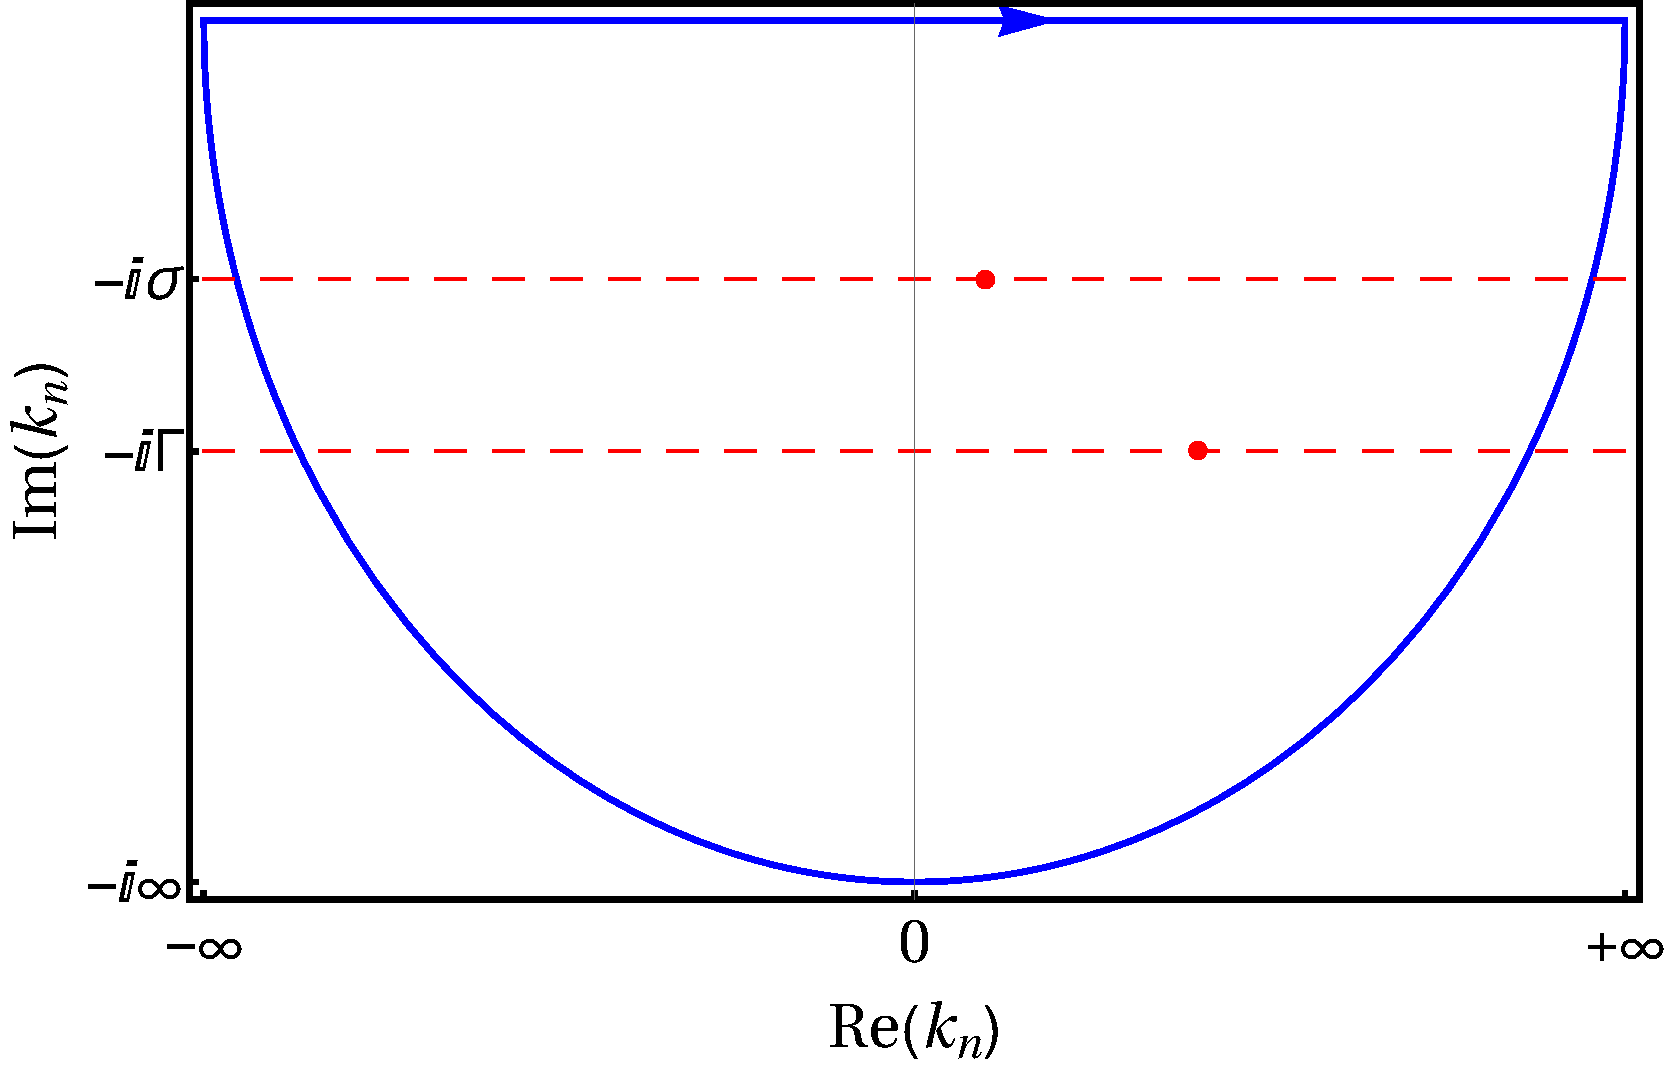
\includegraphics[scale=0.25]{lower_contour.pdf}
%\caption{Integration contour for Eq. (...). The red points are the poles of the
%integrand. The values of the real parts are arbitrary.}
%\label{fig:lower}
%\end{figure}

%\begin{figure}[tbh!]
%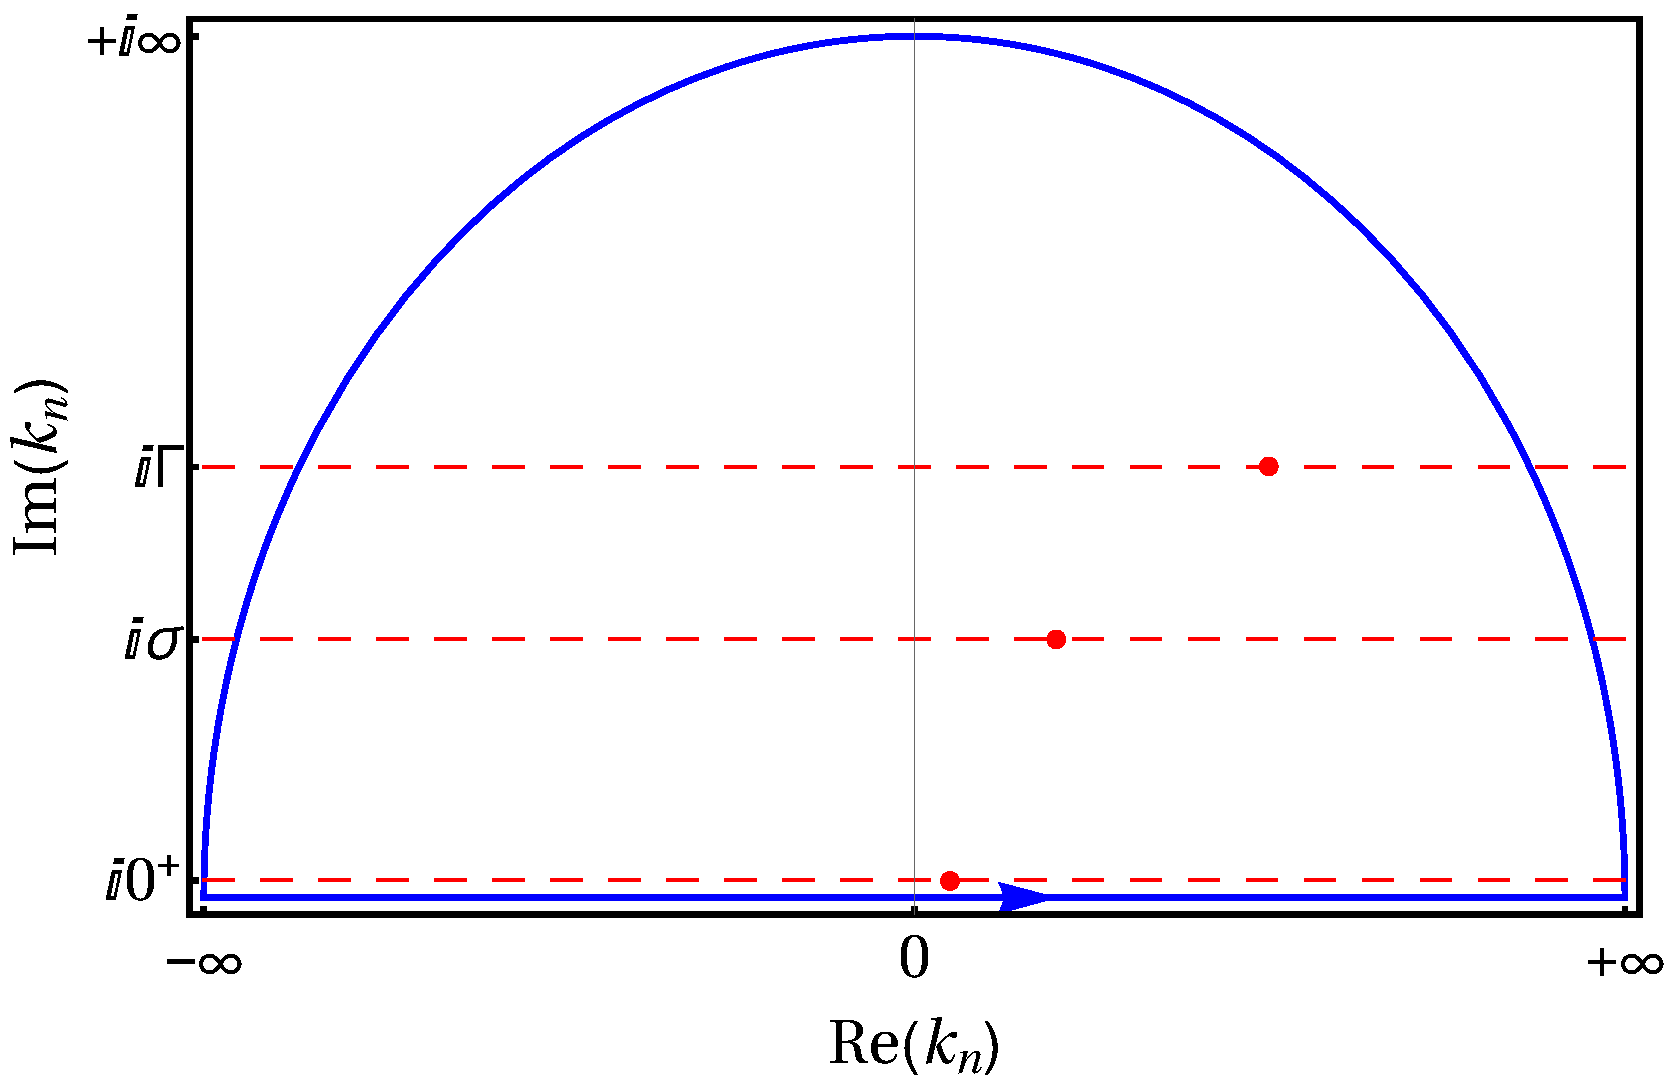
\includegraphics[scale=0.25]{upper_contour.pdf}
%\caption{Integration contour for Eq. (...). The red points are the poles of the
%integrand. The values of the real parts are arbitrary.}
%\label{fig:upper}
%\end{figure}

%\section{Input-output equations for a $\lambda$ atom}
%
%In this section of the Appendix we derive the input-output equations \eqref{eq:a_inout} and \eqref{eq:sigma_inout}. We start from the Hamiltonian for a chiral one-dimensional waveguide coupled to a $\lambda$ atom
%\begin{align}
%H & = \int d\omega \; \omega a_\omega^\dagger a_\omega + E_1\ket{1}\bra{1} + E_2\ket{2}\bra{2} + E_e\ket{e}\bra{e}\nonumber\\
%& + \int d\omega\; (g_1\sigma_{1e}^\dagger a_\omega + g_2 \sigma_{2e}^\dagger a_\omega + \text{H.c.}).
%\end{align}
%%Subtracting $E_1$
%%\begin{align}
%%H & = \int d\omega \; \omega a_\omega^\dagger a_\omega + \Delta_1\sigma_{1e}^\dagger\sigma_{1e} + \Delta_2 \sigma_{2e}^\dagger\sigma_{2e} \nonumber\\
%%& + \int d\omega\; (g_1\sigma_{1e}a_\omega + g_2 \sigma_{2e} a_\omega + \text{H.c.}),
%%\end{align}
%%with $\Delta_\lambda\equiv E_e-E_\lambda$. The operators $\sigma_{\lambda e}=\ket{g_\lambda}\bra{e}$ were defined in the main text (Section \ref{sec:inout}).
%We need to know the Heisenberg equations, $d\mathcal{O}/dt=i[H,\mathcal{O}]$, in order to derive the input-output ones. The Heisenberg equation for $a_\omega(t)$ is
%\begin{equation}\label{eq:aw_Heisenberg}
%i\frac{d a_\omega(t)}{dt}=\omega a_\omega(t) + g_1 \sigma_{1e}(t) + g_2 \sigma_{2e}(t).
%\end{equation}
%For $\sigma_{\lambda e}(t)$
%\begin{align}\label{eq:sigma_Heisenberg}
%&i\frac{d\sigma_{\lambda e}(t)}{dt}=\Delta_\lambda \sigma_{\lambda e}(t)\nonumber\\
%&-\int d\omega\; (g_\lambda \sigma_{\lambda e}^z(t)-g_{\overline{\lambda}} \sigma_{\lambda\overline{\lambda}}(t))a_\omega(t),
%\end{align}
%where the gap $\Delta_\lambda=E_e-E_\lambda$ and the operators $\sigma_{\lambda e}^z=\ket{e}\bra{e}-\ket{g_\lambda}\bra{g_\lambda}$ and $\sigma_{\lambda\overline{\lambda}}=\ket{g_\lambda}\bra{g_{\overline{\lambda}}}$ have already been defined in the main text. As before, $\overline{\lambda}\neq \lambda$.
%
%Evaluationg Eq. \eqref{eq:aw_Heisenberg} at $t=t'$, multiplying it by $e^{i\omega t'}$ and integrating $t'$ from $t_-\to -\infty$ to $t$
%\begin{align}\label{eq:aw_t}
%&a_\omega(t)=e^{-i\omega(t-t_-)} a_\omega(t_-)\nonumber\\
%& - i\sum_{\lambda=1}^2 g_\lambda \int_{t_-}^t dt'\; \sigma_{\lambda e}(t')e^{-i\omega(t-t')}.
%\end{align}
%I define
%\begin{align}
%\label{eq:Phi}\Phi(t) & \equiv \frac{1}{\sqrt{2}}\int d\omega\; a_\omega (t),\\
%a_\text{in}(t) & \equiv \frac{1}{\sqrt{2}}\int d\omega\; a_\omega(t_-) e^{-i\omega(t-t_-)},\\
%a_\text{out}(t) & \equiv \frac{1}{\sqrt{2}}\int d\omega\; a_\omega(t_+) e^{-i\omega(t-t_+)},
%\end{align}
%with $t_\pm\to \pm\infty$. Integrating Eq. \eqref{eq:aw_t} with respect to $\omega$ and taking into account that the decay rates are related to the coupling constants as $\gamma_\lambda=\pi g_\lambda^2$
%\begin{equation}\label{eq:phi_in}
%\Phi(t)=a_\text{in}(t)-i\sum_{\lambda=1}^2\sqrt{\frac{\gamma_\lambda}{2}} \sigma_{\lambda e}(t).
%\end{equation}
%Evaluationg Eq. \eqref{eq:aw_Heisenberg} at $t=t'$, multiplying it by $e^{i\omega t'}$ and integrating $t'$ from $t$ to $t_+\to +\infty$
%\begin{equation}\label{eq:phi_out}
%\Phi(t)=a_\text{out}(t)+i\sum_{\lambda=1}^2\sqrt{\frac{\gamma_\lambda}{2}} \sigma_{\lambda e}(t).
%\end{equation}
%From Eqs. \eqref{eq:phi_in} and \eqref{eq:phi_out}
%\begin{equation}
%a_\text{out}(t)=a_\text{in}(t)-i\sum_{\lambda=1}^2 \sqrt{2\gamma_\lambda} \sigma_{\lambda e}(t),
%\end{equation}
%which is equal to Eq. \eqref{eq:a_inout}. Introducing \eqref{eq:phi_in} in \eqref{eq:sigma_Heisenberg}, taking into account the definition of $\Phi(t)$ \eqref{eq:Phi}
%\begin{align}
%\frac{d\sigma_{\lambda e}(t)}{dt}=&-(i\Delta_\lambda +\gamma_1+\gamma_2)\sigma_{\lambda e}(t)\nonumber\\
%&+i(\sqrt{2\gamma_\lambda} \sigma_{\lambda e}^z(t) - \sqrt{2\gamma_{\overline{\lambda}}}\sigma_{\lambda\overline{\lambda}}(t))a_\text{in}(t),
%\end{align} 
%which is equal to \eqref{eq:sigma_inout}.

\section{Matrix Product States}

As we indicated in the main text, we solve the ultrastrong example by means of the MPS technique. We explain the method and justify why we can use it, as we already did in \cite{Sanchez-Burillo2014,Sanchez-Burillo2015,Sanchez-Burillo2016a}.

Our photonic medium can be treated in the RWA and its ground state is the vacuum both in frequency and position space. Moreover, even if we go beyond RWA in the scatterer-resonator coupling ($g/\Delta\gtrsim 0.1$), it is true that the ground state is not the vacuum anymore, as we showed in \cite{Sanchez-Burillo2014}, but it will follow the area law \cite{Eisert2010}, so it will be slightly entangled. As we are studying the dynamics of two photons flying over the ground state, the state will have a small amount of entanglement.

The main consequence of the previous discussion is that we may use the variational ansatz of Matrix Product States \cite{Ripoll2006,Verstraete2008} to describe the discrete wavefunction, since it is valid for 1D systems when the entanglement is small enough. This ansatz has the form
\begin{equation}
\ket{\psi} = \sum_{s_i \in \{1,d_i\}} \mathrm{tr}\left[
\prod A_i^{s_i}\right] \ket{s_1,s_2,\ldots,s_L}.
\label{eq:mps}
\end{equation}
It is constructed from $L$ sets of complex matrices $A_i^{s_i} \in M[\mathbb{C}^{D}]$, where each set is labeled by the quantum state $s_i$ of the corresponding site. The local Hilbert space dimention $d_i$ is infinity, since we are dealing with bosonic sites. However, during the dynamics, processes creating multiple photons are still highly off-resonance. Thus, we can truncate the bosonic space and consider states with $0$ to
$n_\text{max}$ photons per cavity. So, the composite Hilbert space is $\mathcal{H}=\bigotimes_i \mathbb{C}^{d_i}$, where the dimension is $d_i=n_\text{max}+1$ for the empty resonators and $d_{i_0}=n_\text{scatt}(n_\text{max}+1)$ for the cavity with the scatterer, where $n_\text{scatt}$ is the number of levels of the scatterer. We thus expect the composite wavefunction of the photon-scatterer system to consist of a superposition with a small number of photons

The total number of variational parameters $(L-1)D^2(n_\text{max}+1) + n_\text{scatt}D^2(n_\text{max}+1)$, depends on the size of the matrices, $D$. The key point is that, for describing a general state, $D$ increases exponentially with $L$, whereas its dependence is polynomial if the entanglement is small enough, in such a way that the number of parameters increases polynomially with $L$ for this class of states.

Our work with MPS relies on four different algorithms. The most basic one is to create trivial, product states of known shape, such as a vacuum state with the scatterer in the ground state $\ket{\psi}=\ket{\text{vac}} \ket{g_1}$. These states can be reproduced using matrices of bond dimension $D=1$, so each matrix is just a coefficient $A_i^{s_i}=\delta_{s_i1}$. The second algorithm is to compute expectation values from MPS. This amounts to a contraction of tensors that can be performed efficiently \cite{Ripoll2006}, and allows us to compute single-site operators $\langle a^\dagger_i a_i\rangle$, $\langle \sigma_z\rangle$, or correlators, $\langle a_i^\dagger a_j\rangle$. The third operation that we need to perform is to apply operators on to the state, $\mathcal{O}\ket{\psi}$, such as introducing or removing excitations $a_i^\dagger\ket{\psi}$. We do this in an efficient fashion by interpreting the operator $\mathcal{O}$ as a Matrix Product Operator (MPO) \cite{Pirvu2010}. A MPO is a matrix product representation of an operator:

\begin{equation}
\mathcal{O} = \sum_{s_{i}^{},s_{i}^\prime \in \{1,d_i\}} \mathrm{tr}\left[\prod B_i^{s_i^{},s_i^\prime}\right]\ket{s_1^{},s_2^{},\ldots,s_L^{}}\bra{s_1^\prime,s_2^\prime,\ldots,s_L^\prime}
\end{equation}

So, now we have $L$ sets of complex matrices $B_i^{s_i^{},s_i^\prime} \in M[\mathbb{C}^{D_\mathcal{O}}]$, where each set is labeled by two indices $s_i^{},s_i^\prime$ of the corresponding site.

We just need to apply sums of one-body operators

\begin{equation}
\mathcal{O} = a_\phi^\dagger = \sum_n \phi_n a_n^\dagger.
\end{equation}

In such a case, an efficient representation of the MPO is obtained with $D_\mathcal{O}=2$

\begin{equation}
B_i^{s_i^{},s_i^\prime}=\left(\begin{array}{c c}
\delta_{s_i^{},s_i^\prime} & 0\\
\phi_i(a_i^\dagger)_{s_i^{},s_i^\prime} & \delta_{s_i^{},s_i^\prime}
\end{array}\right)\qquad i=2,3,\dots,L-1,
\end{equation}
whereas $B_1^{s_1^{},s_1^\prime}=(\phi_1(a_1^\dagger)_{s_1^{},s_1^\prime},\delta_{s_1^{},s_1^\prime})$ and $B_L^{s_L^{},s_L^\prime}=(\delta_{s_L^{},s_L^\prime},\phi_L(a_L^\dagger)_{s_L^{},s_L^\prime})^T$, with $(a_i^\dagger)_{s_i^{},s_i^\prime}=:\bra{s_i^{}}a_i^\dagger\ket{s_i^\prime}$.

Finally, with this tool in our box, we can also approximate time evolution, repeatedly contracting the state with an MPO approximation of the unitary operator $\exp(-iH\Delta t)$ for short times, and truncating it to an ansatz with a fixed $D$. Since our problem does not contain long-range interactions and since the state is well approximated by MPS, it is sufficient to rely on a third-order Suzuki-Trotter formula \cite{Suzuki1991}.
In the same way as we can consider time evolution, we can take imaginary time to obtain the ground state and excited states, that is solving the equation $i\tfrac{d}{dt}P\ket{\psi}=PHP\ket{\psi}$ for finite time-steps, while constantly renormalizing the state. Here, $P$ is either the identity (for the ground state) or a projector that either selects a well defined quantum number (parity $\Pi$) or projects out already computed states. In either case, provided a suitable initial state, the algorithm converges to the lowest-energy state of $H$ in the subspace selected by $P$.

\bibliographystyle{apsrev4-1}
\bibliography{bib_cluster}



\end{document}